%% \chapter[htoc-titlei][hhead-titlei]{htitlei}
%% -----------------------------------------------------------------------------
\chapter[Theoretical overview][Theory]{Theoretical overview}
\label{ch:theory}

The universe, as we know it, comprises fundamental matter particles, and
four fundamental forces.
These forces include gravity, electromagnetism, and the strong and weak nuclear
forces.
Despite being the weakest of the four forces, gravity is certainly the most
familiar to everyday life, as it assures objects fall to the ground.
The Gravitational force is described by the general theory of relativity, and
to this day, a successful quantum theory of gravity has yet to be developed.
Since gravity is so weak, it does not significantly affect the physics at the
LHC energy scale, and can safely be ignored for the purpose of this thesis.
Of the remaining three forces,  electromagnetism and the weak force have been
shown to come from the same underlying interactions, called the electroweak
force.
The electroweak and strong forces are described by the Standard Model of
Particle Physics.

In this chapter, a brief overview of the theoretical background for this thesis
is presented.
The Standard Model and its shortcomings are discussed
in \cref{sec:sm,sec:sm_shortcomings}.
Supersymmetry, a popular extension to the Standard Model, is introduced in
Section~\ref{sec:susy}.
The chapter concludes with a presentation of the particular $B-L$ extension to
the SM, which is the focus of the search presented in this dissertation.
Section~\ref{sec:theory_bl_extension} includes presents a brief description of
the underlying theory, as well as some of the interesting phenomenology expected
in the scenario where the scalar top is the LSP.

%% ------------------------------------------------------------------------------
\FloatBarrier
\section{Standard Model}
\label{sec:sm}

In this section, the Standard Model (SM) of particle physics is described in
brief.
The SM is a very rich subject, and a more complete description can be found in
References~\cite{Agashe:2014kda,opac-b1131978,halzen1984quarks}.
The SM is a quantum field theory which encapsulates the current understanding
of the elementary particles, and their interactions, and has been developed,
and rigorously tested by experiments over the last fifty years.
In 2012, the final particle predicted by the SM, the ``Higgs boson`` was
discovered at CERN by the ATLAS and CMS collaborations, marking a great
achievement for the both the experimental collaborations and the theorists
who predicted the particle's existence.
The SM Lagrangian is a non-abelian gauge theory with symmetry group 
$\mathrm{SU}(3)_\mathrm{C} \times
\mathrm{SU}(2)_\mathrm{L} \times
\mathrm{U}(1)_\mathrm{Y}$,
which describes the matter content of the universe, as well as the interactions
of the strong and electroweak forces.
The matter content in the SM is made up of fermions (spin \nicefrac{1}{2}),
called quarks and leptons.
Massless gauge bosons (spin 1) mediate the interactions of the electroweak and
strong forces.

\begin{figure}[ht]
  \centering{
    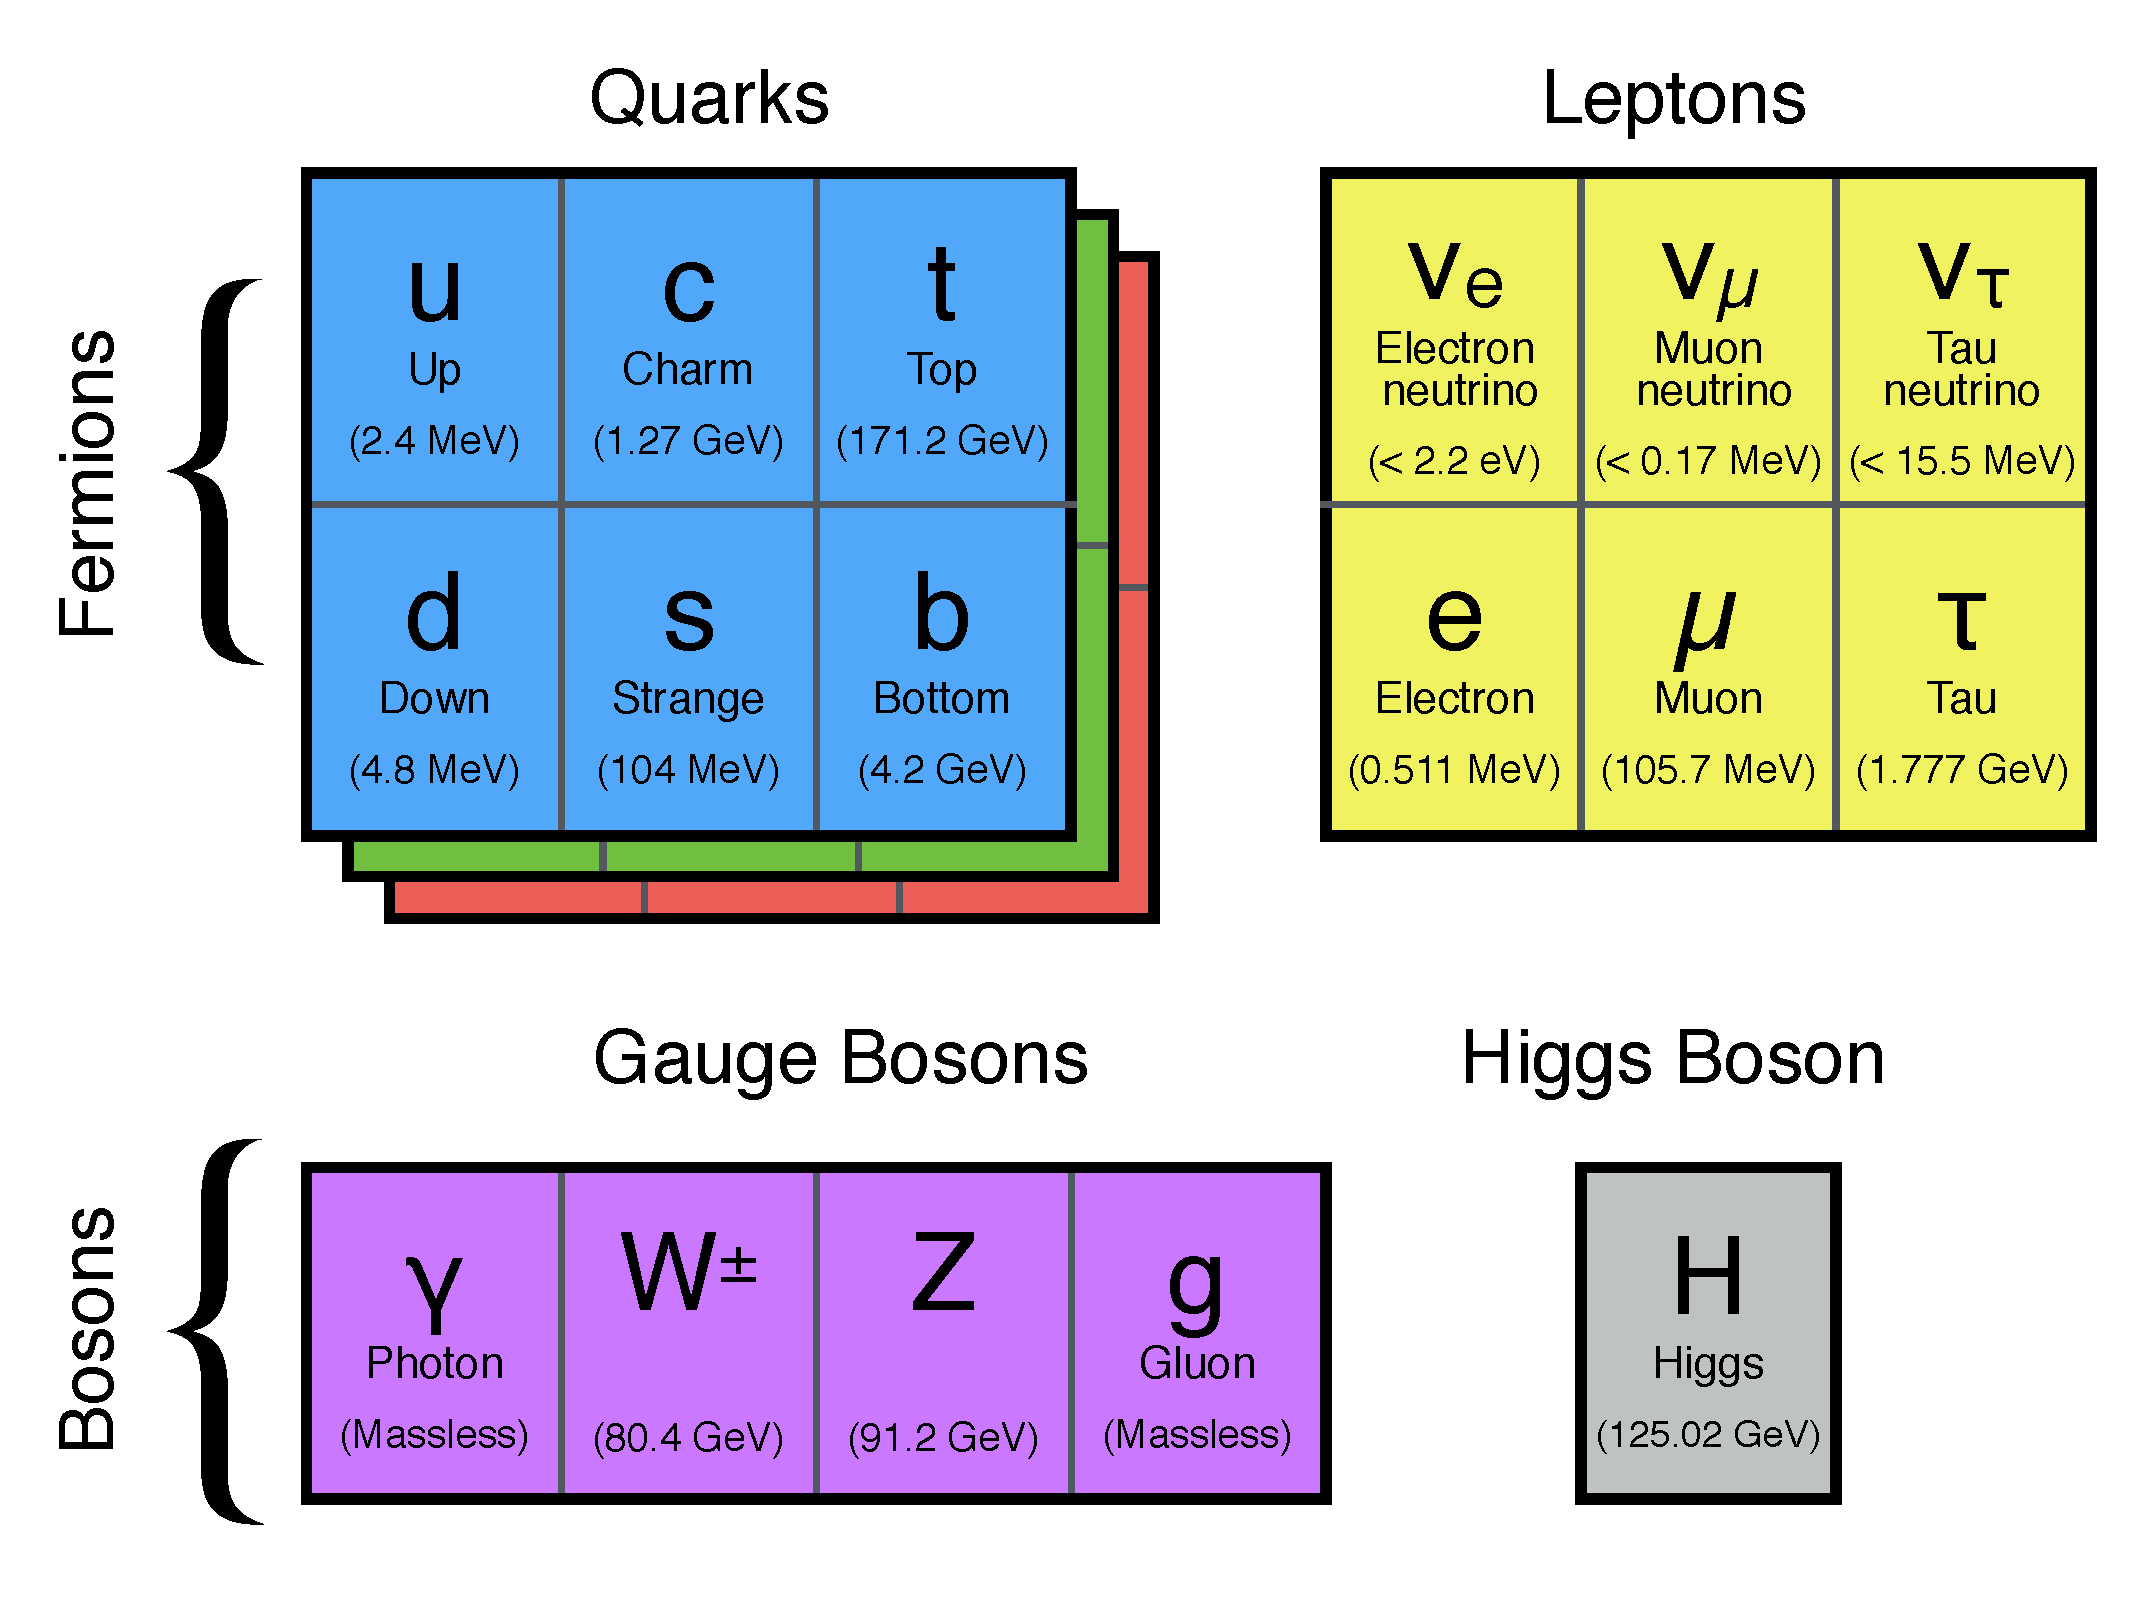
\includegraphics[width=\textwidth]{figs/theory/sm_particle_content.pdf}
    \caption{Fundamental particles described by the Standard Model.
      The masses of each particles are given in parentheses.
    }
    \label{fig:sm_particle_content}
  }
\end{figure}

%% ------------------------------------------------------------------------------
\subsection{Matter}
\label{sec:matter}

The fermionic matter is arranged into three families, or generations, each
containing quarks and leptons.
These particles can be charged under each part of the SM symmetry group,
where the particle's charge determines how it interacts with each of the
corces.
Each generation contains two chiral left-handed quarks, arranged in a isospin
doublet, consisting of an up-type and a down-type quark.
There are also two chiral left-handed leptons, one with electric charge, and
a neutrino, which is electrically neutral.
As with the quarks, the two left-handed leptons are arranged into an isospin
doublet.
Finally, each fermionic family contains chiral right-handed counterparts to
the two quarks, and the charged lepton.
No right-handed neutrinos are included in the SM, as they would no react with
any known forces, as will be explained shortly.
The right-handed fermions are isospin singlets.
The three generations are essentially copies of one another, differing only in
the mass of the constituent particles, and the familiar world is made up
entirely of particles from the first generation.
The reason for exactly three generations, not more or less, remains a mystery.
A summary of the SM matter content, with the charges under the various
parts of the SM symmetry group is shown in Table~\ref{tab:sm_matter_content}.

\begin{table}
  \caption{Summary of the matter particles described by the SM, along with the
    associated quantum numbers.
    The quantum numbers include the spin, electric charge $Q$, the third
    component of weak isospin $T_3$, hypercharge $Y$, and the allowable color
    charges.
  }
  \label{tab:sm_matter_content}
  \begin{center}
    \begin{tabular}{ccccccccc}
      \toprule
      \multirow{2}{*}{Fermions} &
      \multicolumn{3}{c}{Generation} &
      \multirow{2}{*}{Spin} &
      \multirow{2}{*}{$Q$} &
      \multirow{2}{*}{$T_3$} &
      \multirow{2}{*}{$Y$} &
      \multirow{2}{*}{Color}
      \\[1ex]
      & 1 & 2 & 3
      \\
      \midrule
      \addlinespace[1ex]
      %%
      \multirow{5}{*}{Quarks} &
      \multirow{2}{*}{$\left(
        \begin{tabular}{c} u \\ d \end{tabular} \right)_{L}$ } & % (u d) quarks
      \multirow{2}{*}{$\left(
        \begin{tabular}{c} c \\ s \end{tabular} \right)_{L}$ } & % (c s) quarks
      \multirow{2}{*}{$\left(
        \begin{tabular}{c} t \\ b \end{tabular} \right)_{L}$ } & % (t b) quarks
      \multirow{2}{*}{$\frac{1}{2}$} & % Spin
      $+\frac{2}{3}$ & % Q
      $+\frac{1}{2}$ & % T3
      \multirow{2}{*}{$\frac{1}{3}$} & % Y
      \multirow{2}{*}{r, g, b} % color
      \\[1ex]
      %%
      & % Quarks
      & % (u d) quarks
      & % (c s) quarks
      & % (t b) quarks
      & % spin
      $-\frac{1}{3}$ & % Q
      $-\frac{1}{2}$ & % T3
      & % Y
      % color
      \\
      %%
      \cmidrule{2-9}
      %%
      &
      $u_R$ &
      $c_R$ &
      $t_R$ &
      $\frac{1}{2}$ & % spin
      $+\frac{2}{3}$ & % Q
      0 & % T3
      $+\frac{4}{3}$ & % Y
      r, g, b % color
      \\[1ex]
      %%
      &
      $d_R$ &
      $s_R$ &
      $b_R$ &
      $\frac{1}{2}$ & % spin
      $-\frac{1}{3}$ & % Q
      0 & % T3
      $-\frac{2}{3}$ & % Y
      r, g, b % color
      \\
      %%
      \midrule
      %%
      \multirow{3}{*}{Leptons} &
      \multirow{2}{*}{$\left(
          \begin{tabular}{c} $\nu_{e}$ \\ e \end{tabular}
        \right)_{L}$ } &
      \multirow{2}{*}{$\left(
          \begin{tabular}{c} $\nu_{\mu}$ \\ $\mu$ \end{tabular}
        \right)_{L}$ } &
      \multirow{2}{*}{$\left(
          \begin{tabular}{c} $\nu_{\tau}$ \\ $\tau$ \end{tabular}
        \right)_{L}$ } &
      \multirow{2}{*}{$\frac{1}{2}$} & % spin
      0 & % Q
      $+\frac{1}{2}$ & % T3
      \multirow{2}{*}{-1} & % Y
      \multirow{2}{*}{-} % color
      \\[1ex]
      %%
      & % Leptons
      & % (nue e)
      & % (numu mu)
      & % (nutau mu)
      & % spin
      $-1$ & % Q
      $-\frac{1}{2}$ & % T3
      & % Y
      % color
      \\
      \cmidrule{2-9}
      %%
      & % Leptons
      $e_{R}$ &
      $\mu_{R}$ &
      $\tau_{R}$ &
      $\frac{1}{2}$ & % spin
      $-1$ & % Q
      0 & % T3
      $-2$ & % Y
      - % color
      \\
      \bottomrule
    \end{tabular}
  \end{center}
\end{table}

%% ------------------------------------------------------------------------------
\subsection{Quantum electrodynamics}
\label{sec:qed}

In addition to a charge, each piece of the SM symmetry group is associated with
a massless gauge boson, which mediates the interactions between particles.
The electroweak sector has the symmetry group
$\mathrm{SU}(2)_\mathrm{L} \times \mathrm{U}(1)_\mathrm{Y}$, and describes the
interactions with fields with isospin or hypercharge ($Y$) in a theory called
quantum electrodynamics (QED).
The electroweak sector is a chiral theory, meaning right- and left-handed
particles transform differently under the gauge group.
Left-handed fermions have a value of the third component of isospin equal to
$\pm \nicefrac{1}{2}$, while right-handed particles have no isospin, and do
not interact with the weak force.
The gauge bosons associated with the electroweak sector are three $W^{i}$
bosons, arranged in a weak isospin triplet, and a $B^0$ boson, which is a weak
isospin singlet.

Since chiral fields translate differently, depending on their chiral handedness,
there can be no mixing between the right- and left-handed states, which would
break gauge invariance.
Unfortunately, a mass term, allows for exactly this mixing, implying the
fermions, as well as the gauge bosons must be massless.
On the other hand, the weak force is observed to be short ranged, implying
massive gauge bosons, and fermions do indeed have measurable masses.
Adding masses to a chiral quantum field theory is a difficult endeavor, and
is achieved through a process called ``spontaneous symmetry breaking,'' which
is explained in Section~\ref{sec:higgs}.
The broken symmetry leads to a mixing of the $W^3$ and $B^0$ gauge bosons into
a massless photon, and the massive $Z$ boson.
The $W^1$ and $W^2$ become the massive $W^{+}$ and $W^{-}$.
The $W^{\pm}$ and $Z$ bosons both have mass, and act as the propagator of the
weak force, while the massless photon mediates the electromagnetic force.

Since right-handed neutrinos have no charge under any part of the SM symmetry
group, they are not expected to interact with the known components of the SM,
and are therefore not included as part of the theory.
There are extensions to the SM, however, which do include right-handed
neutrinos, including the one described in Section~\ref{sec:theory_bl_extension}.

%% ------------------------------------------------------------------------------
\subsection{Quantum chromodynamics}
\label{sec:qcd}

The $\mathrm{SU}(3)_\mathrm{C}$ part of the SM Lagrangian corresponds to the
strong force, with a corresponding ``color'' charge, and is described by the
theory of quantum chromodynamics (QCD).
Quarks are colored objects, having red, green, or blue charge, while leptons
have no color charge, and thus do not interact directly with the strong
force.
The eight massless gauge bosons associated with the
$\mathrm{SU}(3)_\mathrm{C}$ symmetry group are called gluons, and are
themselves colored objects.
This leads to self interaction, and some interesting phenomenology!

Because the gluon are allowed to interact with one another, QED and QCD have
some very important differences.
Perhaps, the most interesting, is related to the concept of ``screening''.
In QED, as one moves further from a charged paricle, the charge tends to look
smaller as a result of the polarization of the vacuum around the charge, where
electron pairs pop out of the vacuum.
The further from the particle one is, the more electron pairs are visible,
obscuring the initial charge more.
In QCD, this same screening effect occurs, with quark-anti-quark pairs being
pair-produced from the vacuum, however gluon pairs may also be produced out of
the vacuum.
These gluon pairs produce the opposite screening effect, known as
``anti-screening,'' increasing the effective charge observed.
Rather than charges being screened, as in QED, there is a net anti-screening
effect for objects with color charge.

As two colored particles get very close together, the anti-screening is very
small, and they can be treated as free particles, in an effect known as
``asymptotic freedom.''
Alternatively, as two charged particles move apart, the polarization of the
vacuum between them results in an increasing energy buildup, until it is
energetically favorable to pair produce a quark-anti-quark pair from the vacuum.
For this reason, no free quarks or gluons have been observed, rather any
objects with color charge will tend to into bound states called ``hadrons,''
which has no net color.
Hadrons can either be a bound state of a quark-anti-quark pair, called mesons,
or three-quark bound states, called baryons.
The anti-quark contained in a meson must have the corresponding anti-color of 
the constituent quark.
Similarly, the three quarks, which make up a baryon, must have colors that add
to ``white,'' meaning one red , one green, and one blue quark.

In particle collisions, this effect also leads to the phenomenon of ``jets,''
where a spray of hadrons is projected at the particle detector, resulting from
the multiple colored objects being pulled apart due to the energy of the
collision.

%% - - - - - - - - - - - - - - - - - - - - - - - - - - - - - - - - - - - - - - -
\FloatBarrier
\subsection{Brout-Englert-Higgs mechanism}
\label{sec:higgs}

As mentioned in Section~\ref{sec:qed}, the fermions and gauge bosons described
in the SM Lagrangian are massless, however, many of those observed in nature
do, in fact, have a non-negligible mass.
This would seem to allow for the mixing of chiral left- and right-handed
fields, which would in turn break gauge invariance.
A method to add mass terms to the SM Lagrangian without breaking the necessary
gauge invariance was developed during the 1960's by several groups of theorists,
including Robert Brout and Francois Englert~\cite{PhysRevLett.13.321},
Peter Higgs~\cite{Higgs1964132,PhysRevLett.13.508},
and Gerald Guralnik, Carl R. Hagen, and Tom Kibble~\cite{PhysRevLett.13.585}
working in parallel, and is commonly called the Brout-Englert-Higgs (BEH)
mechanism.
The BEH mechanism adds an additional complex scaler field to the Lagrangian,
which acquires a vacuum expectation value (vev), which ``spontaneously''
breaks the symmetry of the SM Lagrangian.

Each spontaneously broken symmetry leads to new massive scalar particle, know
as a ``Goldstone boson.''
The gauge bosons can then absorb these Goldstone bosons in a process where they
acquire a mass.
Recall, before symmetry breaking, the electroweak sector has four massless
gauge bosons, the $W^1$, $W^2$,  $W^3$, and the $B^0$, however experiments
observe massive $W^{\pm}$, and the $Z$ bosons, associated with the weak force,
and a massless photon to mediate the electromagnetic force.
An electric charge $Q$ is also conserved.
This implies that the
$\mathrm{SU}(2)_\mathrm{L} \times \mathrm{U}(1)_\mathrm{Y}$ of QED is broken in
a way that leaves only a $\mathrm{U}(1)_\mathrm{EM}$ symmetry group.
This symmetry breaking requires at least three Goldstone bosons to be absorbed,
and give masses to the gauge bosons.
The simplest method to accomplish this is to add a complex scalar field
\begin{equation}
  \Phi = \begin{pmatrix} \phi^+ \\ \phi^0 \end{pmatrix},
    \label{eqn:scalar_field}
\end{equation}
%which is a doublet with positive hypercharge ($Y=\nicefrac{1}{2}$).
which is a doublet with positive hypercharge ($Y=1$).

To show how this, it is useful to consider the SM Lagrangian, ignoring the
QCD part,
\begin{equation}
  \mathcal{L} =
  - \frac{1}{4} W_{\mu\nu}^{a} W_{a}^{\mu\nu}
  - \frac{1}{4} B_{\mu\nu} B^{\mu\nu}
  + \bar{L}_i \left(i D_{\mu} \gamma^{\mu} \right) L_i
  + \bar{e}_{\mathrm{R},i}\left(i D_{\mu} \gamma^{\mu}\right)e_{\mathrm{R},i},
\end{equation}
where the $i$ index runs over the three generations, the $\mu$,$\nu$ are
Lorentz indices, and $a$ runs over the generators in the gauge group.
The field strengths are given by
\begin{eqnarray}
  W_{\mu\nu}^{a} & = &
  \partial_{\mu}W_{\nu}^{a} - 
  \partial_{\nu}W_{\mu}^{a} +
  g_{2}\epsilon^{abc}W_{\mu}^{b}W_{\nu}^{c}
  \\
  B_{\mu\nu} & = &
  \partial_{\mu}B_{\nu} - 
  \partial_{\nu}B_{\mu},
\end{eqnarray}
and the covariant derivatives for the left- and right-handed lepton fields are
\begin{eqnarray}
  D_{\mu}L_\mathrm{L} & = &
  \left(
    \partial_{\mu} - ig_{2}T_{a}W_{\mu}^{a} - ig_{1}YB_{\mu}
  \right) L_\mathrm{L}
  \\
  D_{\mu}e_\mathrm{R} & = &
  \left(
    \partial_{\mu} - ig_{1}YB_{\mu}
  \right) e_\mathrm{R}.
\end{eqnarray}
$T_a$ are the generators of the gauge group, and $g_1$ and $g_2$ are the
coupling constants for electroweak interactions.

Adding the complex scalar field from Equation~\ref{eqn:scalar_field} adds an
additional scalar part to the Lagrangian,
\begin{equation}
  \mathcal{L} =
  \left(D^{\mu}\Phi\right)^{\dagger}\left(D_{\mu}\Phi\right) - V(\Phi),
  \label{eqn:scalar_lagrangian}
\end{equation}
where the first term is the kinetic term, and $V(\Phi)$ is the scalar
potential.
The exact form of the scalar potential is not known, however, the simplest
possible form that has the desired properties can be used
\begin{equation}
  V(\Phi) = \mu^2 \Phi^{\dagger}\Phi + \lambda\left(\Phi^{\dagger}\Phi\right)^2.
\end{equation}
This form is an assumption that provides the required spontaneous symmetry
breaking, while remaining renormalizable.
In order for the vacuum to be stable, $\lambda$ must be positive.
The choice of the $\mu^2$ parameter affects the shape of the scalar potential,
as shown in Figure~\ref{fig:symmetry_breaking}.
In the configuration with $\mu^2 > 0$, the scalar potential is always positive,
and the minimum occurs at
\begin{equation}
  \bra{0} \Phi \ket{0} = \begin{pmatrix} 0 \\ 0 \end{pmatrix}.
\end{equation}
There is no spontaneous symmetry is this scenario.
On the other hand, if $\mu^2 < 0$, the scalar potential takes on the famous
``Mexican hat'' shape, and the minimum of the potential is no longer located at
the origin.
With the minimum of the scalar potential located away from the origin, the
neutral part of the scalar field acquires a vacuum expectation value (vev) $v$,
\begin{equation}
  \bra{0} \Phi \ket{0} =
  \Phi_0 =
  \frac{1}{\sqrt{2}} \begin{pmatrix} 0 \\ v \end{pmatrix},
  v = \sqrt{\frac{-\mu^2}{\lambda}}.
\end{equation}
By acquiring a vev, electroweak symmetry is spontaneously broken.

\begin{figure}[ht]
  \centering
  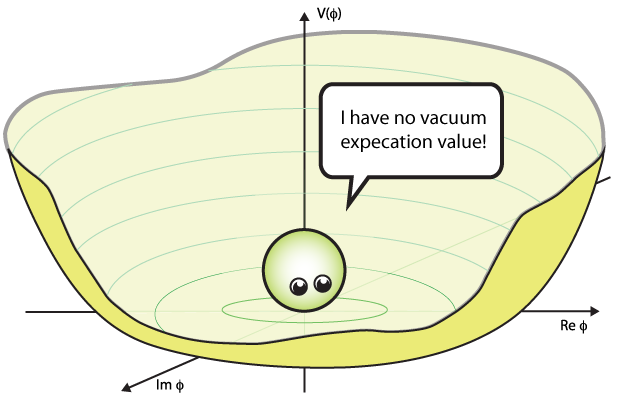
\includegraphics[width=0.48\textwidth]
      {figs/theory/BoringPotential.png}
  \\
  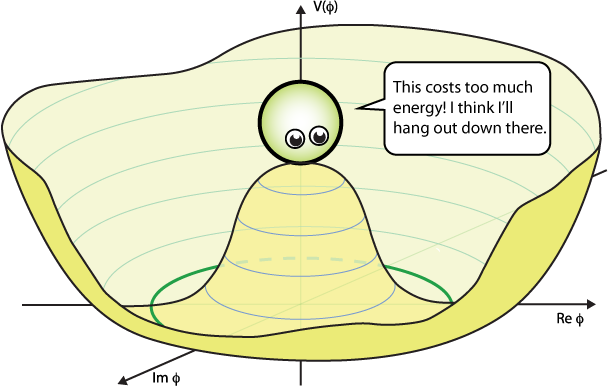
\includegraphics[width=0.48\textwidth]
      {figs/theory/Higgs-Potential-lookdown.png}
  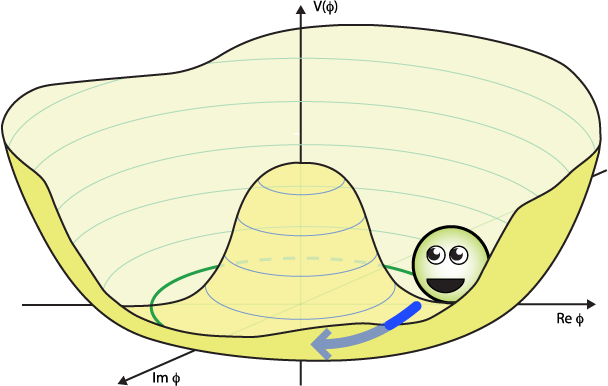
\includegraphics[width=0.48\textwidth]
      {figs/theory/Higgs-Potential-Goldstone.png}
      \caption{The scalar potential under two configurations.
        The configuration on the top shows the case where $\mu^2 > 0$, where
        the scalar potential is always positive.
        In this configuration, the scalar potential has a minimum at the origin.
        The configuration with $\mu^2 < 0$ is shown on the bottom.
        In this case, the minimum of the scalar potential occurs away from the
        origin.
        In this scenario, the scalar field moves away from the origin, in a
        process of spontaneous symmetry breaking.
        The green line corresponds to the circle of minimum potential,
        corresponding to the massless Goldstone
      mode~\cite{QuantumDiariesHiggs}}.
  \label{fig:symmetry_breaking}
\end{figure}

Since the charged part of the scalar field does not acquire a vev,
electromagnetism is not broken, leaving a remaining $U(1)_\mathrm{EM}$
symmetry with a conserved charge of
\begin{equation}
  Q = T_3 + \frac{Y}{2},
\end{equation}
corresponding to the electric charge.

Expanding the scalar field $\Phi$ around it's minimum $\Phi_0$, one gets
\begin{equation}
  \Phi(x) = \frac{1}{\sqrt{2}} \begin{pmatrix} 0 \\ v + h(x) \end{pmatrix},
\end{equation}
with $h(x)$ being a new scalar field.
Inserting this into the kinetic term of Equation~\ref{eqn:scalar_lagrangian},
and redefining the gauge fields as
\begin{eqnarray}
  W_{\mu}^{\pm} & = & \frac{1}{\sqrt{2}}
                      \left( W_{\mu}^{1} \mp W_{\mu}^{2} \right),
  \\
  Z_{\mu} & = & \frac{1}{\sqrt{g_1^2 + g_2^2}}
                \left( g_2 W_{\mu}^{3} - g_1 B_{\mu} \right),
  \\
  A_{\mu} & = & \frac{1}{\sqrt{g_1^2 + g_2^2}}
                \left( g_2 W_{\mu}^{3} + g_1 B_{\mu} \right),
\end{eqnarray}
where the redefined gauge fields correspond to the physical gauge bosons
of QED, the $W^{\pm}$, $Z$, and the photon.
The covariant derivative becomes
\begin{equation}
  \left| D_{\mu}\Phi \right|^2 =
  \frac{1}{2} \left( \partial_{\mu} H \right)^2 +
  \frac{1}{2} g_{2}^{2} \left(v + H\right)^2 W_{\mu}^{+}W^{\mu -} +
  \frac{1}{8} \left(v + H\right)^2 \left(g_{1}^{2} + g_{2}^{2} \right)
    Z_{\mu}Z^{\mu}.
\end{equation}
It can be seen that the gauge bosons take on the following masses through their
interactions with the scalar field
\begin{eqnarray}
  M_{W} &=& \frac{1}{2} v g_2 \\
  M_{Z} &=& \frac{1}{2} v \sqrt{g_1^2 + g_2^2} \\
  M_{A} &=& 0
\end{eqnarray}
It is important to note that there is no term for the photon, implying it does
not interact with the scalar field, and therefore, does not pick up a mass
term.
Three of the degrees of freedom from the scalar field that would be Goldstone
bosons have been absorbed by the gauge bosons, giving them mass.
There is one remaining degree of freedom, which becomes the Higgs boson.
The Higgs boson itself has mass, equal to
\begin{eqnarray}
  m_H &=& 2 \lambda v^2 \\
      &=& 2\mu^2.
\end{eqnarray}
This mass corresponds to the remaining degree of freedom in the scalar
potential, where the field can oscillate in the radial direction, as shown in
Figure~\ref{fig:higgs_mass}.
The Higgs mass has no other handles in the SM, and must be determined
experimentally.
It was found to be equal to
$125.02^{+0.22}_{0.27}\mathrm{(stat)}^{+0.14}_{-0.15}\mathrm{(syst)} \GeV$
by the ATLAS and CMS experiments.

\begin{figure}[ht]
  \centering
  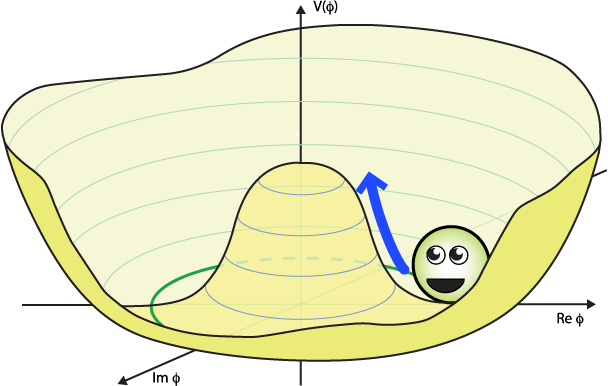
\includegraphics[width=0.48\textwidth]{figs/theory/Higgs-Potential-radial.png}
  \caption{The Higgs boson corresponds to an excitation in the radial direction
    of the scalar potential~\cite{QuantumDiariesHiggs}.
  }
  \label{fig:higgs_mass}
\end{figure}

The final piece to add to the SM are masses for the fermions, which are
introduced through Yukawa cuplings between the fermion fields and the scalar
field.
An additional set of terms are added to the Lagrangian for the interactions
between the scalar field and the fermion sector.
The portion that represents the first generation of fermions is
\begin{equation}
  \mathcal{L}_\mathrm{F} =
  - G_e \bar{L} \Phi e_\mathrm{R}
  - G_d \bar{Q} \Phi d_\mathrm{R}
  - G_u \bar{Q} \tilde{\Phi} u_\mathrm{R}
  + \mathrm{h.c.}.
  \label{eqn:fermion_lagrangian}
\end{equation}
There are copies of these terms for the second and third generations of
fermions.
A new term, $\tilde{\Phi}$ was introduced, which is the conjugate of $\Phi$
with negative hypercharge ($Y = 1$), and is equal to
\begin{eqnarray}
  \tilde{\Phi} &=& i \tau_2 \Phi^{*} \\
               &=& \frac{1}{\sqrt{2}} \begin{pmatrix} v + h \\ 0 \end{pmatrix}.
\end{eqnarray}
Substituting terms into Equation~\ref{eqn:fermion_lagrangian} gives
\begin{align}
  \begin{split}
    \mathcal{L}_\mathrm{F} =
      - \frac{1}{\sqrt{2}}
      &
      \left[
      G_e
    \begin{pmatrix} \bar{\nu} & \bar{e} \end{pmatrix}_\mathrm{L}
    \begin{pmatrix} 0 \\ v+h \end{pmatrix}
      e_\mathrm{R}
      %% 
      + G_d
    \begin{pmatrix} \bar{u} & \bar{d} \end{pmatrix}_\mathrm{L}
    \begin{pmatrix} 0 \\ v+h \end{pmatrix}
      d_\mathrm{R}
      \right.
      \\
      &
      \left.
      %%
      + G_u
    \begin{pmatrix} \bar{u} & \bar{d} \end{pmatrix}_\mathrm{L}
    \begin{pmatrix} v+h \\ 0 \end{pmatrix}
      u_\mathrm{R}
    \right]
    %%
    + \mathrm{h.c.}
    %%
  \end{split}
\end{align}
%%
\begin{equation}
  \mathcal{L}_\mathrm{F} =
  - \frac{1}{\sqrt{2}}
  (v+h)
  \left(
    G_e \bar{e}_\mathrm{L} e_\mathrm{R} +
    G_d \bar{d}_\mathrm{L} d_\mathrm{R} +
    G_u \bar{u}_\mathrm{L} u_\mathrm{R}
  \right) + \mathrm{h.c.}.
  \label{eqn:expanded_fermion_lagrangian}
\end{equation}

Generic fermion mass terms are of the form
$m \bar{f}_\mathrm{L} f_\mathrm{R} + \mathrm{h.c.}$, so reading
Equation~\ref{eqn:expanded_fermion_lagrangian}, one can see the fermion masses
are
% \begin{align}
%   \begin{split}
%     m_e = & \frac{G_e v}{\sqrt{2}} \\
%     m_u = & \frac{G_u v}{\sqrt{2}} \\
%     m_d = & \frac{G_d v}{\sqrt{2}}.
%   \end{split}
% \end{align}
\begin{equation}
    m_e = \frac{G_e v}{\sqrt{2}},~~~~~
    m_u = \frac{G_u v}{\sqrt{2}},~~~~~
    m_d = \frac{G_d v}{\sqrt{2}}.
\end{equation}
The $h$ is dropped because it is the remnant of the Higgs doublet, and expected
to be negligible.
There are of course similar mass terms for the second and third generation
fermions.
Since the neutrinos have no isospin, they do not interact with the scalar
potential, and therefore, do not pick up a mass.
It should also be noted that the $G$'s, thus the fermion masses, are not
predicted by the SM, and the fermion masses must be measured, and inputed
into the theory.

%% -----------------------------------------------------------------------------
\FloatBarrier
\section{Shortcomings}
\label{sec:sm_shortcomings}

While the SM has been a very successful theory in describing particles
and their interactions across many orders of magnitude, it does have some
shortcomings.
Some of these shortcomings, such as the existence of dark matter arise from
experimental observations, which point toward potential problems with the SM,
and currently constructed.
Others, such as the Hierarchy problem arise from parts of the SM, which seem
to require, seemingly unnatural, amounts of ``fine tuning'' of the parameters
of the theory.

%% -----------------------------------------------------------------------------
\FloatBarrier
\subsection{Gravity}

One (seemingly obvious) feature, missing from the SM is the gravitational
force.
This seems counterintuitive because this is probably the force people are most
familiar with, in their daily lives.
However, gravity remains a very weak force, compared to the electroweak scale,
and no successful quantum theory of gravity has been created.
A spin 2 graviton particle has been proposed, which seems as if it can be added
to the SM, but experiments have yet to observe such a particle.

%% -----------------------------------------------------------------------------
\FloatBarrier
\subsection{Dark matter and dark energy}

Cosmological experiments over the past several
decades\cite{Clowe:2006eq,Ade:2013zuv} have shown that observable matter
only makes up 5\% of the observable universe.
It is still unknown what makes up the remaining 95\%!
The unknown component is generally broken up into two categories, based on
their expected properties.
Dark matter is localized, and tends to be found in clumps, while dark energy
permeates all of space.

From the perspective of gravity, dark matter is expected to behave similar to
normal matter, in that gravity exerts an attractive force on the dark matter.
Dark matter differs in that it does not interact with electromagnetism,
which is why it is called ``dark.''
The other properties of dark matter are unknown.
It is possible that it interacts with the strong or weak forces, however, this
is by no means guaranteed.

Dark energy, on the other hand, opposed the force of gravity, applying a
repulsive force, accelerating the expansion of the universe.

%% -----------------------------------------------------------------------------
\FloatBarrier
\subsection{Neutrino masses}

As shown in Section~\ref{sec:higgs}, the BEH mechanism leaves the neutrinos
massless in the SM because they have no chiral right-handed counterpart, and
don't generate the Yukawa coupling with the scalar field.
Neutrino experiments, have observed neutrino flavor oscillation, suggesting
they do, in fact, have a mass~\cite{PhysRevD.86.010001}.
For these oscillations to occur, the physical neutrino eigenstates must be
a mixture of the flavor eigenstates, and have distinct masses.
This provides evidence that there is a non-zero mass for at least two of the
three neutrino masses.
Some of the proposed mechanisms to generate massive neutrino masses with the
SM are the addition of ``sterile'' right-handed neutrinos, or the possibility
that neutrinos are Majorana particles, and they are their own anti-particle.

%% -----------------------------------------------------------------------------
\FloatBarrier
\subsection{Hierarchy problem}

Several potential problems arises from the large differences in energy scale
between the electroweak scale ($\mathcal{O}(100)~\GeV$), where experiments are
able to effectively probe, and the Planck scale ($\mathcal{O}(10^{18})~\GeV$),
where the effects of gravity can no longer be ignored, and the theory is no
longer valid as it stands.
Because the scales are so different, the bare parameters of the theory can
differ from their renormalized values, or other values in the theory,
by several orders of magnitude.
These problems are classified as ``hierarchy problems,'' and do not immediately
lead to contradictions, as the theory can remain consistent with these large
differences.
However, in order to construct a consistent theory, one is required to accept
a certain amount of ``fine tuning,'' that many find unsatisfying.

A particularly famous hierarchy problem is associated with the mass of the
Higgs boson.
Observed particles masses are a combination of the ``bare'' mass (tree level)
and radiative corrections from additional loop diagrams.
The one-loop corrections to the Higgs mass are shown in
Figure~\ref{fig:oneloopdiagrams}.
These loop momenta are cut off at the Planck scale, which leaves a lot of room
for the these radiative corrections to increase.
Fermion and gauge boson masses are protected from this high cutoff scale.
Fermions are protected through chiral symmetry, and are only logarithmically
dependent on the cutoff scale. 
Gauge bosons are similarly protected through the local gauge symmetry.
The Higgs boson is a scalar, and has a quadratic dependence on the cutoff
scale.
This tends to push the mass much higher than the weak scale.

The Higgs mass is observed to be at 125~\GeV, so if the bare mass and the
radiative correction terms are truly at such a high scale, it would be a large
coincidence if they simply happen to cancel so precisely.
While it is not impossible, it is extremely unlikely this would happen.
This is the essence of the fine tuning problem.

A way to remove the quadratic dependence on the Planck scale is to introduce
new particles, which have the opposite loop behavior to their SM counterparts.
This is the basic idea of supersymmetry, which is discussed in
Section~\ref{sec:susy}.

\begin{figure}[t]
  \begin{tikzpicture}[scale=0.9]
    \node[void] (in) at (0,0)  {};
    \node[void] (v1) at (1,0) {};
    \node[void] (v2) at (2,0) {};
    \node[void] (out) at (3,0) {};
    \draw[spin0] (in) -- node [above]{$H$} (v1) ;
    \draw (1.5,0) circle (0.5);
    \node at (1.5,0.7) {$f$};
    \draw[spin0] (v2) -- node [above]{$H$} (out);
  \end{tikzpicture}
  \hfill
  \begin{tikzpicture}[scale=0.9]
    \node[void] (in) at (0,0)  {};
    \node[void] (v1) at (1,0) {};
    \node[void] (v2) at (2,0) {};
    \node[void] (out) at (3,0) {};
    \draw[massvect] (v1) arc(180:0:0.5) ;
    \node at (1.5,0.8) {$W,Z$};
    \draw[spin0] (in) -- node [above]{$H$} (v1) -- (v2) -- node [above]{$H$} (out);
  \end{tikzpicture}
  \hfill
  \begin{tikzpicture}[scale=0.9]
    \node[void] (in) at (0,0)  {};
    \node[void] (v1) at (1,0) {};
    \node[void] (v2) at (2,0) {};
    \node[void] (out) at (3,0) {};
    \draw[massvect] (1.5,0.45) circle (0.5);
    \node at (1.5,1.3) {$W,Z$};
    \draw[spin0] (in) -- node [above]{$H$} (v1) -- (v2) -- node [above]{$H$} (out);
  \end{tikzpicture}
  \hfill
  \begin{tikzpicture}[scale=0.9]
    \node[void] (in) at (0,0)  {};
    \node[void] (v1) at (1,0) {};
    \node[void] (v2) at (2,0) {};
    \node[void] (out) at (3,0) {};
    \draw[spin0] (1.5,0.5) circle (0.5);
    \node at (1.5,1.3) {$H$};
    \draw[spin0] (in) -- node [above]{$H$} (v1) -- (v2) -- node [above]{$H$} (out);
  \end{tikzpicture}
  \caption{One-loop quantum corrections to the Higgs boson mass.
    From left to right: contribution
    from the Yukawa interaction; two contributions from the gauge interaction;
    contribution from the Higgs self-interaction.
  }
  \label{fig:oneloopdiagrams}
\end{figure}

%% -----------------------------------------------------------------------------
\FloatBarrier
\section{Supersymmetry}
\label{sec:susy}

Supersymmetry (SUSY) is a popular extension to the SM that describes the
interactions between the fermions and bosons with a quantum field
theory~\cite{Miyazawa:1966,PhysRev.170.1586,Volkov:1972jx,Volkov:1973ix,
  Volkov:1973jd,Ramond:1971gb,Golfand:1971iw,Neveu:1971rx,Neveu:1971iv,
  Gervais:1971ji,Wess:1973kz,Wess:1974tw}.
The idea behind SUSY was first proposed by Miyazawa, in 1966, to relate
mesons and baryons in the context of hadronic
physics.
During the early 1970s, it was independently rediscovered in the context of
quantum field theory by several research groups.
In this case, SUSY acts as a new spacetime symmetry relating the fermions and
the bosons within the theory.
SUSY is also needed for grand unified theories and string theories, where it is
necessary to have a link between particles of different spin.

%% -----------------------------------------------------------------------------
\FloatBarrier
\subsection{Motivation}
\label{sec:susy_motivation}

A new operator $Q$ is defined to generate the transformations of fermions into
bosons and conversely bosons into fermions.
\begin{align}
  \begin{split}
    Q\ket{\mathrm{fermion}} & = \ket{\mathrm{boson}} \\
    Q\ket{\mathrm{boson}}   & = \ket{\mathrm{fermion}}
  \end{split}
\end{align}
Since $Q$ transforms a field between fermionic and bosonic states, it must
have spin \nicefrac{1}{2}.
The operator also has the following commutation and anti-commutation
relationships
\begin{align}
  \begin{split}
    \{Q, Q^{\dagger}\} & = P^{\mu} \\
    \{Q, Q\}           & = \{Q^{\dagger}, Q^{\dagger}\} = 0 \\
    [Q, P^{\mu}]       & = [Q^{\dagger}, P^{\mu}] = 0,
  \end{split}
\end{align}
where $P^{\mu}$ is the generator of spacetime transformations.

The particles are now arranged in ``supermultiplets,'' each containing a
fermion and a boson.
Another effect of adding the $Q$ generator is new particle content, in addition
to the SM particles, is added to the theory.
Each supermultiplet contains one SM particle and one new field, and $Q$
translates between the two fields within a particular multiplet.
$Q$ and $Q^{\dagger}$ commute with generators of the gauge transformations,
so the particles within a supermultiplet have the same gauge transformations.
This implies, the supersymmetric partners undergo the same interactions as
their SM counterparts, with the same coupling strengths.
$Q$ and $Q^{\dagger}$ also commute with $P^2$, which implies the supersymmetric
partners have the same mass as the SM particles.
This is clearly not the case, as SUSY has not yet been observed at these low
mass scales; thus, if supersymmetry is a real symmetry of nature, it must be
a broken symmetry.

Despite being a broken symmetry, SUSY has some nice features, providing
potential solutions to some of the shortcomings of the SM listed in
Section~\ref{sec:sm_shortcomings}.
\begin{description}
  \item[Hierarchy problem] \hfill \\
    The hierarchy problem may be addressed by
    supersymmetry through the addition of new, massive particles which enter
    loop diagrams of the Higgs boson.
    These new particles provide radiative corrections to the Higgs mass which
    have opposite sign compared to the corrections from their SM counterparts.
    These radiative corrections can provide a cutoff scale, removing the
    quadratic dependence on the Planck scale, preventing the Higgs mass from
    becoming too large.
  \item[Dark matter] \hfill \\
    The SM does not include any particles with the
    properties necessary to describe the dark matter content of the universe.
    By adding new, massive particles, SUSY can potentially offer a dark matter
    candidate.
    In many SUSY models, the lightest supersymmetric particle (LSP) is massive,
    stable, and has no electric charge.
    These are exactly the properties needed by a dark matter candidate!
    Even in models where the LSP is unstable, its lifetime may be long enough
    to be consistent with a dark matter particle.
\end{description}

%% - - - - - - - - - - - - - - - - - - - - - - - - - - - - - - - - - - - - - - -
\FloatBarrier
\subsection{Formalism}
\label{sec:susy_formalism}
In this section, the formalism of SUSY is briefly introduced.
A more complete discussion of the formalism is provided in
References~\cite{aitchison2007supersymmetry,Martin:1997ns,Polonsky:2001pn}.

Within the supersymmetry framework, the fields representing the matter
particles and force propagators of the SM are placed into supermultiplets,
along with their supersymmetric counterparts, which have a spin differing
by \nicefrac{1}{2}, but otherwise the same quantum numbers.
These supermultiplets, therefore, have one fermion and one boson each.
Rather than formulating interactions between the fields directly, the
supersymmetric Lagrangian formulates interactions between superfields,
resulting in several new terms.

The supermultiplets take on two forms.
The simplest form including a two-component Weyl fermion and a complex scalar
field, and is called a ``chiral'' or ``matter'' superfield.
This class of supermultiplets describes the SM fermions, along with their
supersymmetric partner, the scalar fermion (sfermion).
The scalar Higgs fields also form these types of supermultiplets.
Unlike the case of fermions, however, the Higgs fields have spin-0, and their
partners, the higgsino, are fermions, with spin-\nicefrac{1}{2}.
It should be noted that, the left- and right-handed fermions reside in
different multiplets.
For this reason, the sfermions are assigned a ``handedness'' even though
the concept of handedness is somewhat ambiguous for a scalar particle.
In this case, it simply refers to the handedness of the fermionic partner.

The second class of supermultiplets, called a ``gauge'' or ``vector''
multiplet, and includes a spin-1 gauge boson, and a massless
spin-\nicefrac{1}{2} Weyl fermion.
The supersymmetric partners of the gauge bosons are fermions are called
gauginos, and transform the same as their boson counterparts under gauge
transformations.
Therefore, the left- and right-handed gauginos are in the same supermultiplet.

As mentioned in Section~\ref{sec:susy_motivation}, no supersymmetric particles
have been observed with the same mass as their SM counterparts; for this
reason, if SUSY is a true symmetry of nature, it must be a broken.
In order to solve the hierarchy problem, only soft SUSY breaking is allowed,
otherwise, quadratic divergences reappear.
This means that the relation between dimensionless coupling constants must
still hold.
This leaves only logarithmically diverging terms of the form
\begin{equation}
  \Delta m_{H}^2 =
  m_\mathrm{soft}^2
  \left(
    \frac{\lambda}{16\pi^2}
    \ln \frac{\Lambda}{m_\mathrm{soft}}
    + ...
  \right),
\end{equation}
If the masses of the supersymmetric partners become too large,
$m_\mathrm{soft}$ is related to the masses of the supersymmetric partners, so
the corrections to the Higgs mass become large again, reintroducing the
hierarchy problem.
This suggests that, at least some of the new particles must be light to avoid
the fine-tuning of the hierarchy problem.

%% - - - - - - - - - - - - - - - - - - - - - - - - - - - - - - - - - - - - - - -
\FloatBarrier
\subsection{Minimal supersymmetric Standard Model}
\label{sec:mssm}

In order to construct a supersymmetric Standard Model (MSSM), the SM particles
must be placed into the context of supersymmetric multiplets.
As discussed in Section~\ref{sec:susy_formalism}, there are two types of
supermultiplets which can be used to construct the model, chiral superfields,
and gauge superfields.
The SM fermions transform differently under the gauge transformations depending
on the chirality (left- or right- handedness); for this reason, the SM fermions
must be placed into chiral supermultiplets, where the left- and right-handed
particles are treated separately.
The supersymmetric partners of the fermions have spin-0, and are called
scalar fermions, or sfermions.
As with the SM fermions, the sfermions are made up of the partners come in
two types, called scalar quarks (squarks), which have color charge, and scalar
leptons (sleptons), which do not interact with the strong force.
As the names suggest, the squarks and sleptons are the supersymmetric
counterparts of the SM quarks and leptons.
Despite the fact that these sfermions are scalar particles, they are assigned
a handedness, corresponding to the handedness of the SM counterpart.
This should not be confused with the particles being truly left- or
right-handed chiral fields.

The gauge bosons have spin-1, and are placed in gauge supermultiplets with
their supersymmetric partners, the gauginos.
The gauginos have spin-\nicefrac{1}{2}, and are fermions.
Unlike the SM fermions however, the gauginos transform the same as the gauge
bosons under gauge transformations in a way that does not depend on the
handedness of the particle.

The Higgs boson is the final particle to include in this MSSM.
Since the Higgs boson is a scalar, it must be placed into a chiral
supermultiplet, with a fermion Higgsino.
It should be noted that in the supersymmetric model, a single Higgs boson is
not sufficient, and a second chiral Higgs supermultiplet is added.
A second supermultiplet is necessary in a due to the basic structure of
supersymmetric models and to cancel anomalies that arise due to the additional
symmetry breaking.
\begin{description}
  \item[Structure] \hfill \\
    In the SM, the scalar field gives mass to the
    up-type quarks and the conjugate field gives mass to the down-type quarks
    and charged leptons.
    In supersymmetric models, the Higgs field has hypercharge
    $Y=+\nicefrac{1}{2}$, and gives mass to the up-type quarks, however the
    conjugate of the Higgs field no longer gives mass to the particles with
    negative hypercharge.
    A second scalar field with hypercharge $Y=-\nicefrac{1}{2}$ is added to
    give masses to the down-type quarks and the charged leptons
  \item[Anomaly cancellation] \hfill \\
    In general, breaking a gauge symmetry of the Lagrangian can introduce
    anomalies, and cause the theory to be inconsistent.
    While the SM has several broken symmetries, it remains a consistent theory
    because it satisfies the condition
    $\Tr\left[ T_3^2 Y \right] = \Tr\left[ Y^3 \right] = 0$, where the trace
    is run over the left-handed Weyl fermionic degrees of freedom.
    If a single Higgsino field, with either $Y=+\nicefrac{1}{2}$ or
    $Y=-\nicefrac{1}{2}$ is added to the theory, the cancellation is broken,
    and the theory becomes inconsistent.
    Adding a second Higgsino field with the opposite hypercharge restores the
    cancellation.
\end{description}
The two Higgsino fields in the MSSM are named $H_\mathrm{u}$ and $H_\mathrm{d}$,
and have $Y=+\nicefrac{1}{2}$ and $Y=-\nicefrac{1}{2}$ respectively.
The subscript represents the types of quark which interact with the Higgsino
field.

The full list of chiral and gauge supermultiplets contained in the MSSM are
shown in \cref{tab:chiral_superfields,tab:gauge_superfields}.
It should also be noted that, just as the $W^3$ and $B$ fields of the SM mix to
form the photon and the $Z$ boson, the corresponding gauginos mix to form the
zino ($\tilde{Z}$) and the photino ($\tilde{\gamma}$).

\begin{table}[ht]
  \caption{Chiral supermultiplet fields in the
    MSSM~\cite{aitchison2007supersymmetry}.
  }
  \label{tab:chiral_superfields}
  \begin{center}
    \begin{tabular}{ccccc}
      \toprule
      \multicolumn{2}{l}{Names} &
      Spin 0 &
      Spin \nicefrac{1}{2} &
      $\mathrm{SU}(3)_\mathrm{C},
       \mathrm{SU}(2)_\mathrm{L},
       \mathrm{U}(1)_\mathrm{Y}$ \\
      \midrule
      %%
      Squarks, quarks&
      $Q$ &
      $\left( \tilde{u}_\mathrm{L}, \tilde{d}_\mathrm{L} \right)$ &
      $\left( u_\mathrm{L}, d_\mathrm{L} \right)$ &
      $\mathbf{3}, \mathbf{2}, \nicefrac{1}{3}$ \\[1ex]
      %%
      (3 families) &
      $\bar{u}$ &
      $\tilde{\bar{u}}_\mathrm{L} = \tilde{u}_\mathrm{R}^{\dagger}$ &
      $\bar{u}_\mathrm{L} = \left( u_\mathrm{R} \right)^\mathrm{c}$ &
      $\mathbf{3}, \mathbf{1}, -\nicefrac{4}{3}$ \\[1ex]
      %%
      &
      $\bar{d}$ &
      $\tilde{\bar{d}}_\mathrm{L} = \tilde{d}_\mathrm{R}^{\dagger}$ &
      $\bar{d}_\mathrm{L} = \left( d_\mathrm{R} \right)^\mathrm{c}$ &
      $\mathbf{3}, \mathbf{1}, \nicefrac{2}{3}$ \\
      %%
      \midrule
      %%
      Sleptons, leptons &
      $L$ &
      $\left( \tilde{\nu}_{e, \mathrm{L}}, \tilde{e}_\mathrm{L} \right)$ &
      $\left( nu_{e, \mathrm{L}}, e_\mathrm{L} \right)$ &
      $\mathbf{1}, \mathbf{2}, -1$ \\[1ex]
      %%
      (3 families) &
      $\bar{e}$ &
      $\tilde{\bar{e}}_\mathrm{L} = \tilde{e}_\mathrm{R}^{\dagger}$ &
      $\bar{e}_\mathrm{L} = \left( e_\mathrm{R} \right)^\mathrm{c}$ &
      $\mathbf{1}, \mathbf{1}, 2$ \\
      %%
      \midrule
      Higgs, Higgsinos &
      $H_\mathrm{u}$ &
      $\left( H_\mathrm{u}^{+}, H_\mathrm{u}^{0} \right)$ &
      $\left( \tilde{H}_\mathrm{u}^{+}, \tilde{H}_\mathrm{u}^{0} \right)$ &
      $\mathbf{1}, \mathbf{2}, 1$ \\[1ex]
      %%
      &
      $H_\mathrm{d}$ &
      $\left( H_\mathrm{d}^{0}, H_\mathrm{d}^{-} \right)$ &
      $\left( \tilde{H}_\mathrm{d}^{0}, \tilde{H}_\mathrm{d}^{-} \right)$ &
      $\mathbf{1}, \mathbf{2}, -1$ \\
      %%
      \bottomrule
    \end{tabular}
  \end{center}
\end{table}

\begin{table}[ht]
  \caption{Gauge supermultiplet fields in the
    MSSM~\cite{aitchison2007supersymmetry}.
  }
  \label{tab:gauge_superfields}
  \begin{center}
    \begin{tabular}{cccc}
      \toprule
      Names &
      Spin \nicefrac{1}{2} &
      Spin 1 &
      $\mathrm{SU}(3)_\mathrm{C},
       \mathrm{SU}(2)_\mathrm{L},
       \mathrm{U}(1)_\mathrm{Y}$ \\
      \midrule
      %%
      Gluinos, gluons &
      $\tilde{g}$ &
      $g$ &
      $\mathbf{8}, \mathbf{1}, 0$ \\[1ex]
      %%
      Wino, $W$ boson &
      $\tilde{W}^{\pm}, \tilde{W}^{0}$ &
      $W^{\pm}, W^{0}$ &
      $\mathbf{1}, \mathbf{3}, 0$ \\[1ex]
      %%
      Bino, $B$ boson &
      $\tilde{B}$ &
      $B$ &
      $\mathbf{1}, \mathbf{1}, 0$ \\
      %%
      \bottomrule
    \end{tabular}
  \end{center}
\end{table}

%% - - - - - - - - - - - - - - - - - - - - - - - - - - - - - - - - - - - - - - -
\FloatBarrier
\subsection{Supersymmetric Lagrangian}
\label{sec:mssm_lagrangian}

In constructing a supersymmetric model, a new Lagrangian is constructed, with
kinetic and interaction terms.
The kinetic terms of a supersymmetric Lagrangian are of the form
\begin{equation}
  \mathcal{L}_\mathrm{kinetic} =
  - \frac{1}{4} G_{\mu\nu}^{a} G_{a}^{\mu\nu}
  + \tilde{G}^{\dagger a} i \bar{\sigma}^{\mu} D_{\mu} \tilde{G}_{a}
  + f^{\dagger i} i \bar{\sigma}^{\mu} D_{\mu} f_{i}
  - \left( D_{\mu} \phi_{i} \right)^{\dagger} D^{\mu} \phi^{i},
\end{equation}
where $G$ and $\tilde{G}$ represent any gauge boson and gaugino in the theory
respectively.
$f$ is any fermion, and $\phi$ is any scaler field.

The interaction terms are written in terms of a superpotential $\mathcal{W}$,
and takes the form.
\begin{equation}
  \mathcal{L}_\mathrm{int} =
  - \sum_{i} \left| \frac{\partial \mathcal{W}}{\partial z_i} \right|^2
  - \frac{1}{2} \sum_{ij}
  \left( \bar{f}_i \frac{\partial^2 \mathcal{W}}{\partial z_i \partial z_j} f_j
  + \mathrm{h.c.} \right).
  %%
  \label{eqn:mssm_lagrange_int}
\end{equation}
$z_i$ are the superfields of theory, and the theory is specified by
$\mathcal{W}$.
The particular form of $mathcal{W}$ that leads to the MSSM is 
\begin{equation}
  \mathcal{W} =
  \sum_{ij}
  \left(
    - Y_{ij}^\mathrm{u} \bar{u}_i H_\mathrm{u} \cdot Q_j
    + Y_{ij}^\mathrm{d} \bar{d}_i H_\mathrm{d} \cdot Q_j
    + Y_{ij}^{\ell}     \bar{e}_i H_\mathrm{d} \cdot Q_j
    + \mu H_\mathrm{u} \cdot H_\mathrm{d}
  \right),
\end{equation}
where $Y_{ij}$ are Yukawa couplings among generations, and superscript is a
label for the type of interaction rather than an index to be summed over.
First three terms are generalizations of SM Yukawa interactions.
Last term is globally supersymmetric mass for the Higgs fields.

%% - - - - - - - - - - - - - - - - - - - - - - - - - - - - - - - - - - - - - - -
\FloatBarrier
\subsection{R-Parity}
\label{sec:r_parity}

The extension of the Standard Model of particle physics with supersymmetry
immediately leads to processes that violate both baryon number ($B$) and
lepton number ($L$).
In addition to the interaction terms given in
Equation~\ref{eqn:mssm_lagrange_int}, the most general MSSM Lagrangian may
contain terms such as
\begin{align}
  % \begin{split}
    W_{\Delta L = 1} & =
    \frac{1}{2} \lambda^{ijk} L_{i} L_{j} \bar{e}_{k} +
    \lambda'^{ijk} L_{i} Q_{j} \bar{d}_{k} +
    \mu'^{i} L_{i} H_\mathrm{u},
    \label{eqn:rpv_terms_1}
    \\
    %%
    W_{\Delta B = 1} & =
    \frac{1}{2} \lambda''^{ijk} \bar{u}_{i} \bar{d}_{j} \bar{d}_{k},
    \label{eqn:rpv_terms_2}
  % \end{split}
\end{align}
where $i$, $j$, $k$ indicate the family indices.
If both the lepton number violating and baryon number violating terms are
allowed to contribute, the interactions lead to rapid proton decay
($p \to \pi^{0} e^{+}$, and lepton-number-violating processes, such
as unseen decays of $\mu \to e\gamma$, in conflict with experimental bounds.
A conventional assumption to prevent these processes is to impose
conservation of $R$-parity~\cite{Fayet:1976et,Fayet:1977yc,Farrar:1978xj,
Fayet:1979sa,Dimopoulos:1981zb},
defined as
\begin{equation}
  R=(-1)^{3(B-L)+2s},
\end{equation}
where $s$ is the spin of the particle.
This has a value of $+1$ for Standard Model particles and $-1$ for
SUSY particles.
In this case SUSY particles are produced in pairs, and the LSP is stable.
Further, this stable LSP cannot carry electric charge or color charge without
coming into conflict with astrophysical data.
A stable LSP also serves as a viable dark matter candidate.
At the LHC, the conventional experimental signature for SUSY particles
includes significant missing transverse momentum due to the non-interaction of
the LSP with the detector.

%% -----------------------------------------------------------------------------
\FloatBarrier
\section{B-L extension}
\label{sec:theory_bl_extension}

While $R$-Parity conservation does prevent the rapid decay of the proton, it is
a rather strict requirement.
There exist alternative approaches, that accomplish the same goal, but allow
for some of the interactions described in
Equations~\ref{eqn:rpv_terms_1}~and~\ref{eqn:rpv_terms_2}.
One such approach is to add a local symmetry $\mathrm{U}(1)_{B-L}$ to the
$\mathrm{SU}(3)_\mathrm{C} \times
\mathrm{SU}(2)_\mathrm{L} \times
\mathrm{U}(1)_\mathrm{Y}$ SM with right-handed neutrinos.
The minimal supersymmetric extension then only needs a vacuum expectation value
for a right-handed sneutrino in order to spontaneously break the
$B-L$ symmetry~\cite{FileviezPerez:2008sx, Barger:2008wn, FileviezPerez:2009gr,
Everett:2009vy, Evans:1986ada, Lukas:1998yy, Braun:2005ux, Braun:2005nv,
Braun:2006ae, Ambroso:2009jd, Ambroso:2010pe, Ovrut:2012wg}.
This minimal $B-L$ model violates lepton number but not baryon number, and is
consistent with proton stability and the bounds on lepton number violation.
The LSP can now decay via $R$-parity-violating (RPV) processes, and may now
carry color and electric charge.

%% - - - - - - - - - - - - - - - - - - - - - - - - - - - - - - - - - - - - - - -
\FloatBarrier
\subsection{Phenomenology}

This leads to unique signatures~\cite{FileviezPerez:2012mj, Perez:2013kla,
Ovrut:2012wg, Ovrut:2014rba, Ovrut:2015uea} that are disallowed in conventional
models with $R$-parity conservation.
The case where the LSP is a scalar top (stop) is most interesting
since, in general, the large mass of the top quark acts to make the
lightest stop significantly lighter than the other squarks due to
renormalization group effects~\cite{Barbieri:1987fn,deCarlos:1993yy}.
The stop decays via an RPV interaction to a charged lepton (of any
flavor) and a $b$-quark.
The decay branching fractions to $e b$, $\mu b$, and $\tau b$ may be different,
in a manner related to the neutrino mass
hierarchy seen in Figure~\ref{fig:pheno_bounds}.
Each point in this plot represents a simulation with a particular choice of
model parameters, all varied within a natural range of values, shown in
Table~\ref{tab:pheno_ranges}, and the four colors represent different choices
for the neutrino mass hierarchy and 
$\sin^2\theta_{23}$~\cite{Marshall:2014cwa,Marshall:2014kea}.
There is a clear relation between the neutrino mass hierarchy and the allowed
stop branching ratios, therefore if a stop consistent with this model is
discovered, its properties could potentially give information about the
structure of the neutrino sector.

\begin{figure}[p]
  \centering{
    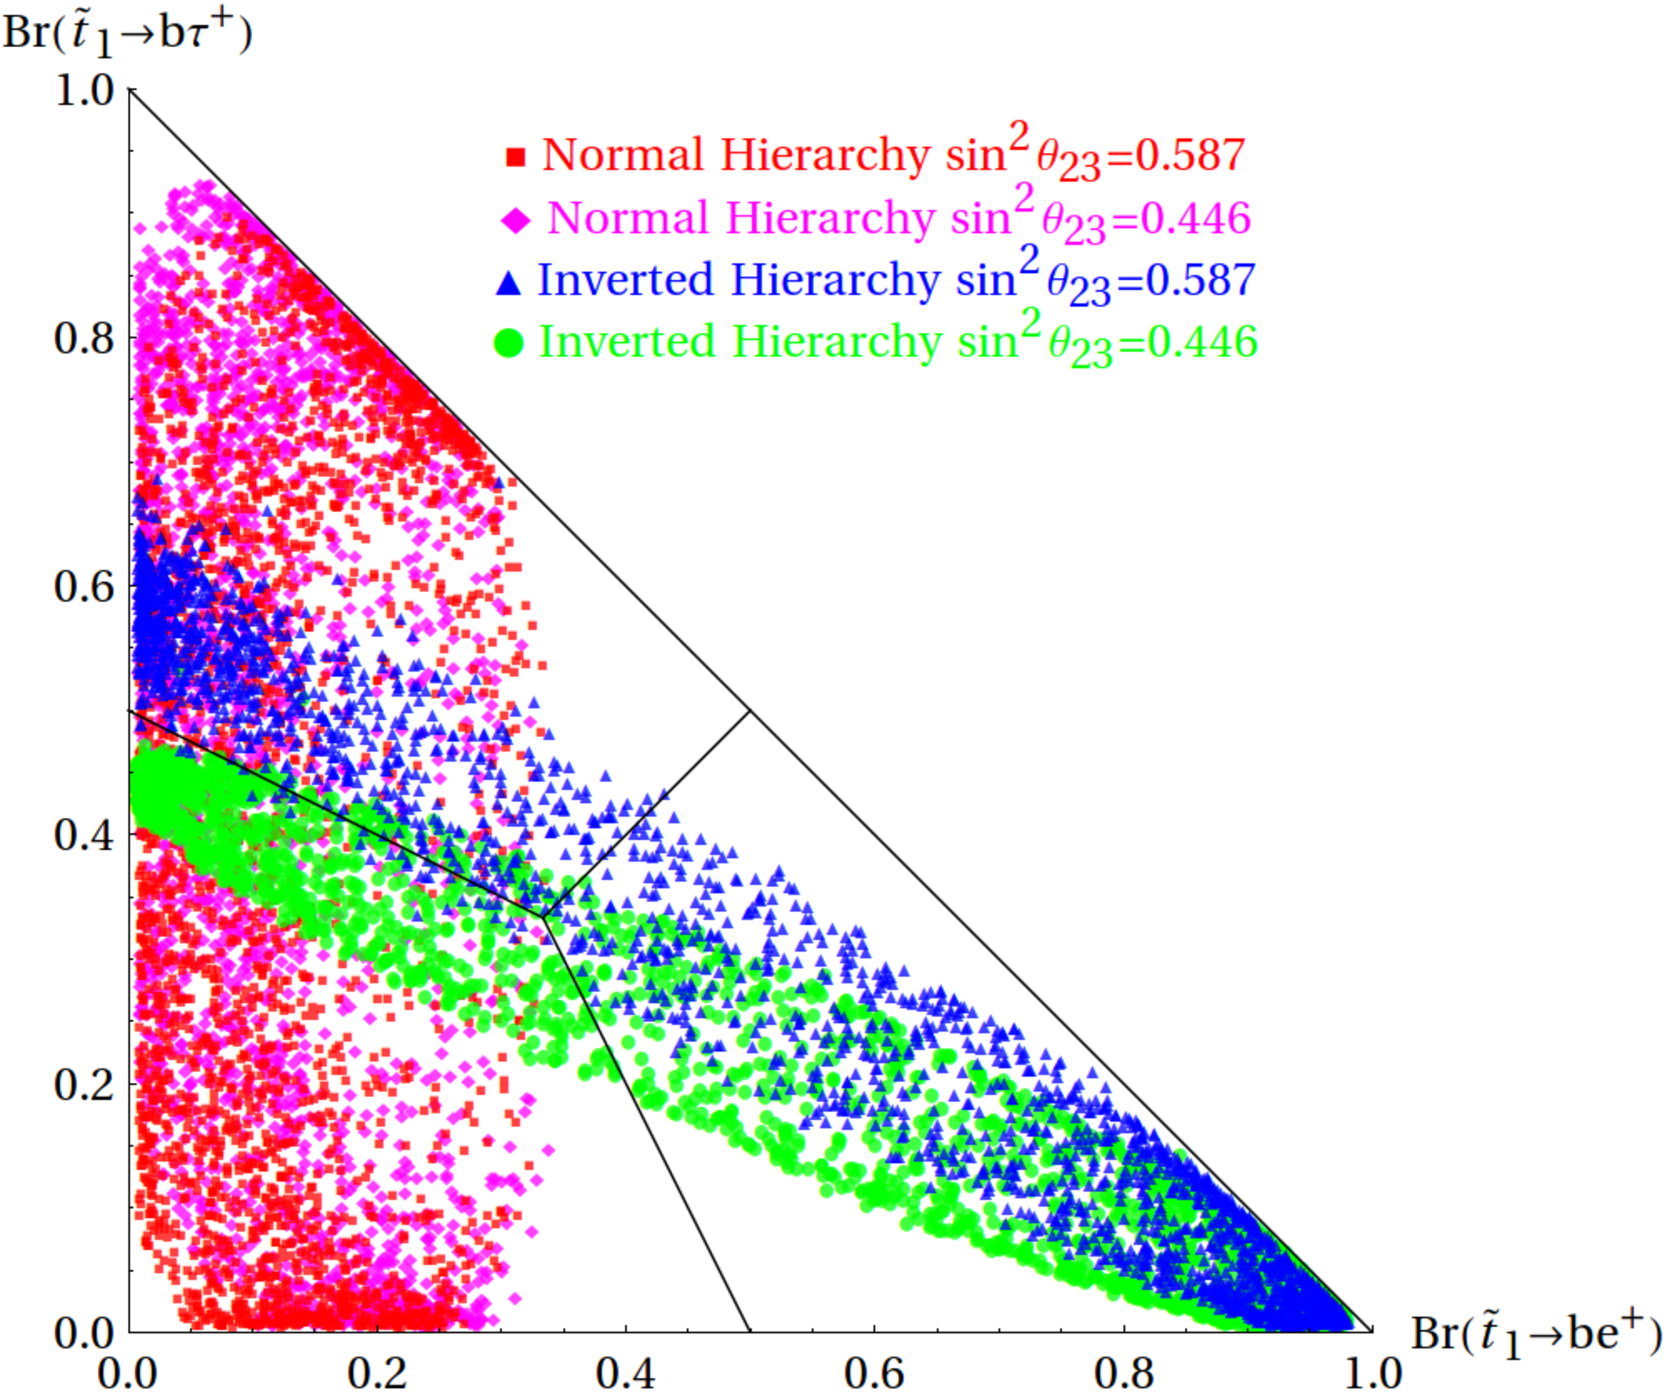
\includegraphics[width=\textwidth]{figs/theory/WithGaussian.pdf}
    \caption{This plot shows the allowed branching ratios for the stop LSP
      for various choices of the neutrino mass hierarchy and
      $\sin^2\theta_{23}$,
      obtained by varying various model parameters within a range of natural
      values shown in Table~\ref{tab:pheno_ranges}~\cite{Marshall:2014cwa}.
    }
    \label{fig:pheno_bounds}
  }
\end{figure}

\begin{table}[ht]
  \caption{Ranges for the parameter scan used to generate the simulated models
    in \cref{fig:stop_vs_mixing_angle,fig:pheno_bounds}.
    The neutrino sector constrains all buy one one of the R-parity violating
    parameters, which is chosen to be $\epsilon_i$ where the generational
    index, $i$, is also scanned to avoid any biases.
    ``NH'' and ``IH'' represent the normal and inverted neutrino mass hierarchy
    respectively~\cite{Marshall:2014cwa}.
  }
  \label{tab:pheno_ranges}
  \centering{
    \begin{tabular}{cc}
      \toprule
      Parameter & Range \\
      \midrule
      $M_3~[\TeV]$               & $1.5 - 10$    \\[1ex]
      $M_{Z_\mathrm{R}}~[\TeV]$  & $2.5 - 10$    \\[1ex]
      $\tan\beta$                & $2 - 55$      \\[1ex]
      $\mu~[\GeV]$               & $150 - 1000$  \\[1ex]
      $m_{\stop_1}~[\GeV]$       & $400 - 1000$  \\[1ex]
      $\theta_t~[^\circ]$        & $0 - 90$      \\[1ex]
      $|\epsilon_i|~[\GeV]$      & $10^{-4} - 1$ \\[1ex]
      $\arg(\epsilon_i)$         & $0 - 360$     \\[1ex]
      $i$                        & $1 - 3$       \\[1ex]
      $\xi_0, \xi_3$             & $-1, 1$       \\[1ex]
      $\delta,\alpha~[^{\circ}]$ & $0 - 360$     \\[1ex]
      Neutrino Hierarchy         & NH, IH        \\
      \bottomrule
    \end{tabular}
  }
\end{table}

Within this model, a stop LSP can decay in one of two ways, depending on
the handedness of the stop.
A right-handed stop decays to a top quark and a right-handed neutrino with a
coupling strength proportional to vacuum expectation value (VEV) of the
left-handed neutrino mass.
This must be small because the left-handed sneutrino interacts with the
$W$ and $Z$ bosons, and a large VEV would result in these bosons gaining
additional mass.
{\color{red} (TODO check this statement is true - I think I'm missing
something).}
A purely left-handed stop decays to a $b$-quark and a lepton with the coupling
strength proportional to the VEV of the right-handed sneutrino, which may be
large, as the right-handed sneutrino does not couple to the electroweak bosons,
a large VEV does not break electroweak symmetry.
{\color{red} (TODO check this statement is true - I think I'm missing
something)}.
In the scenario where the stop LSP is an admixture of left- and right-handed
stops, the preferred decay mode depends on the stop mixing angle ($\theta_t$).
This dependence is plotted in Figure~\ref{fig:stop_br_vs_mixing_angle}, which
shows the ratio
$\nicefrac{\mathrm{Br}(\stop \to t\nu)}{\mathrm{Br}(\stop \to b\ell)}$
versus $\theta_t$.
Each point represents a simulation with a particular choice of model parameters,
again scanning over the natural values in Table~\ref{tab:pheno_ranges}.
The $\stop \to b\ell$ decay is the dominant decay mode for mixing angles less
than abut $80^{\circ}$, where the LSP stop is mostly right handed, and the
$\stop \to t\nu$ decay becomes significance.
The $\stop \to b\ell$ decay is still non-negligible for a mostly right-handed
stop in many of the simulated models,
however~\cite{Marshall:2014cwa,Marshall:2014kea}.

\begin{figure}[ht]
  \centering{
    \subbottom[Stop branching ratio]{
      % 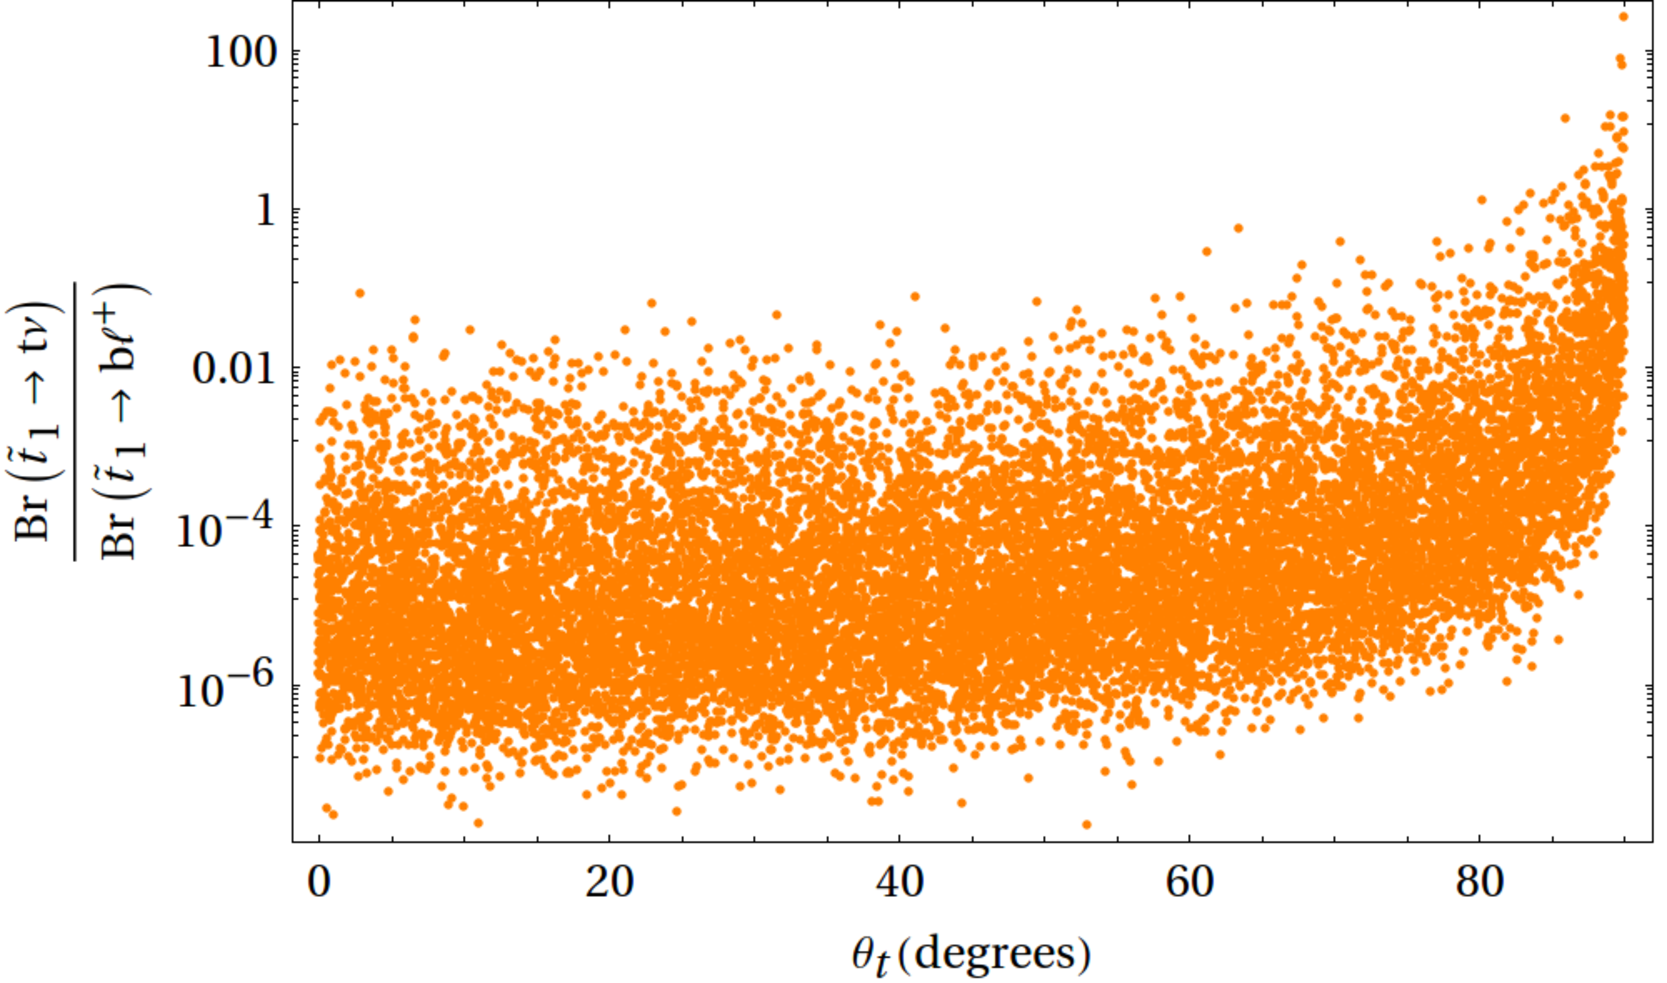
\includegraphics[width=0.70\textwidth]{figs/theory/StopBranchingRatiosVsMixingAngle.pdf}
      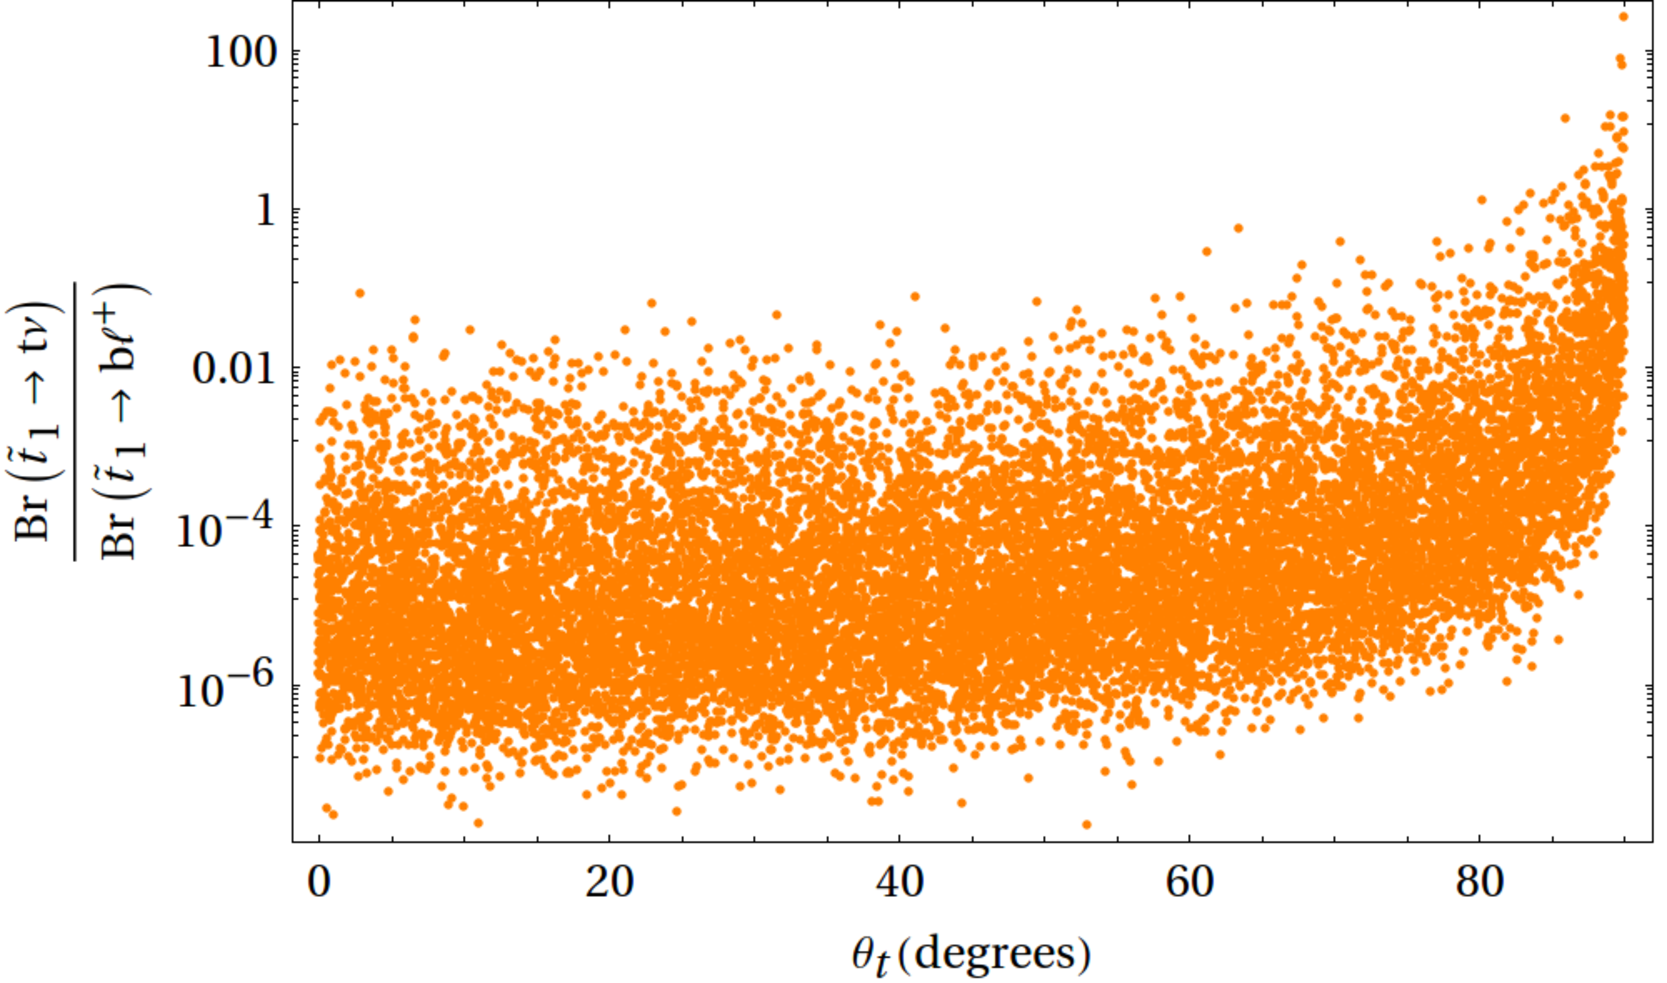
\includegraphics[width=\textwidth]{figs/theory/StopBranchingRatiosVsMixingAngle.pdf}
      \label{fig:stop_br_vs_mixing_angle}
    }
    \subbottom[Stop decay length]{
      % 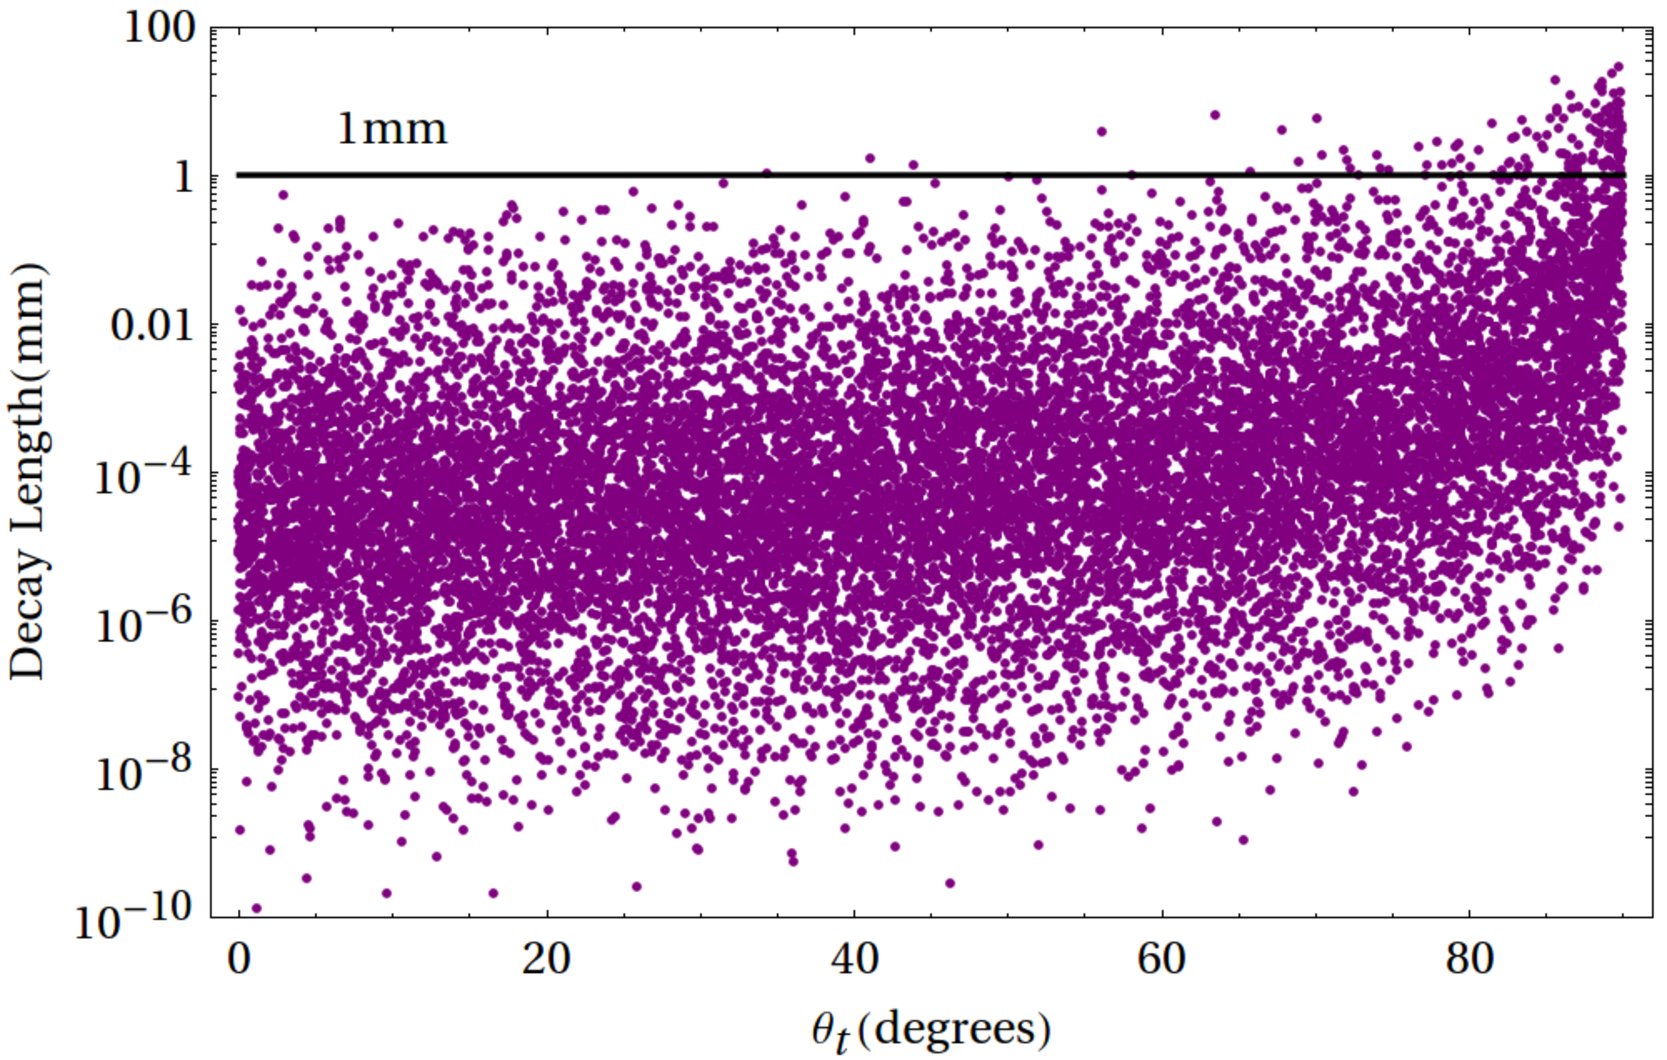
\includegraphics[width=0.70\textwidth]{figs/theory/DecayLength.pdf}
      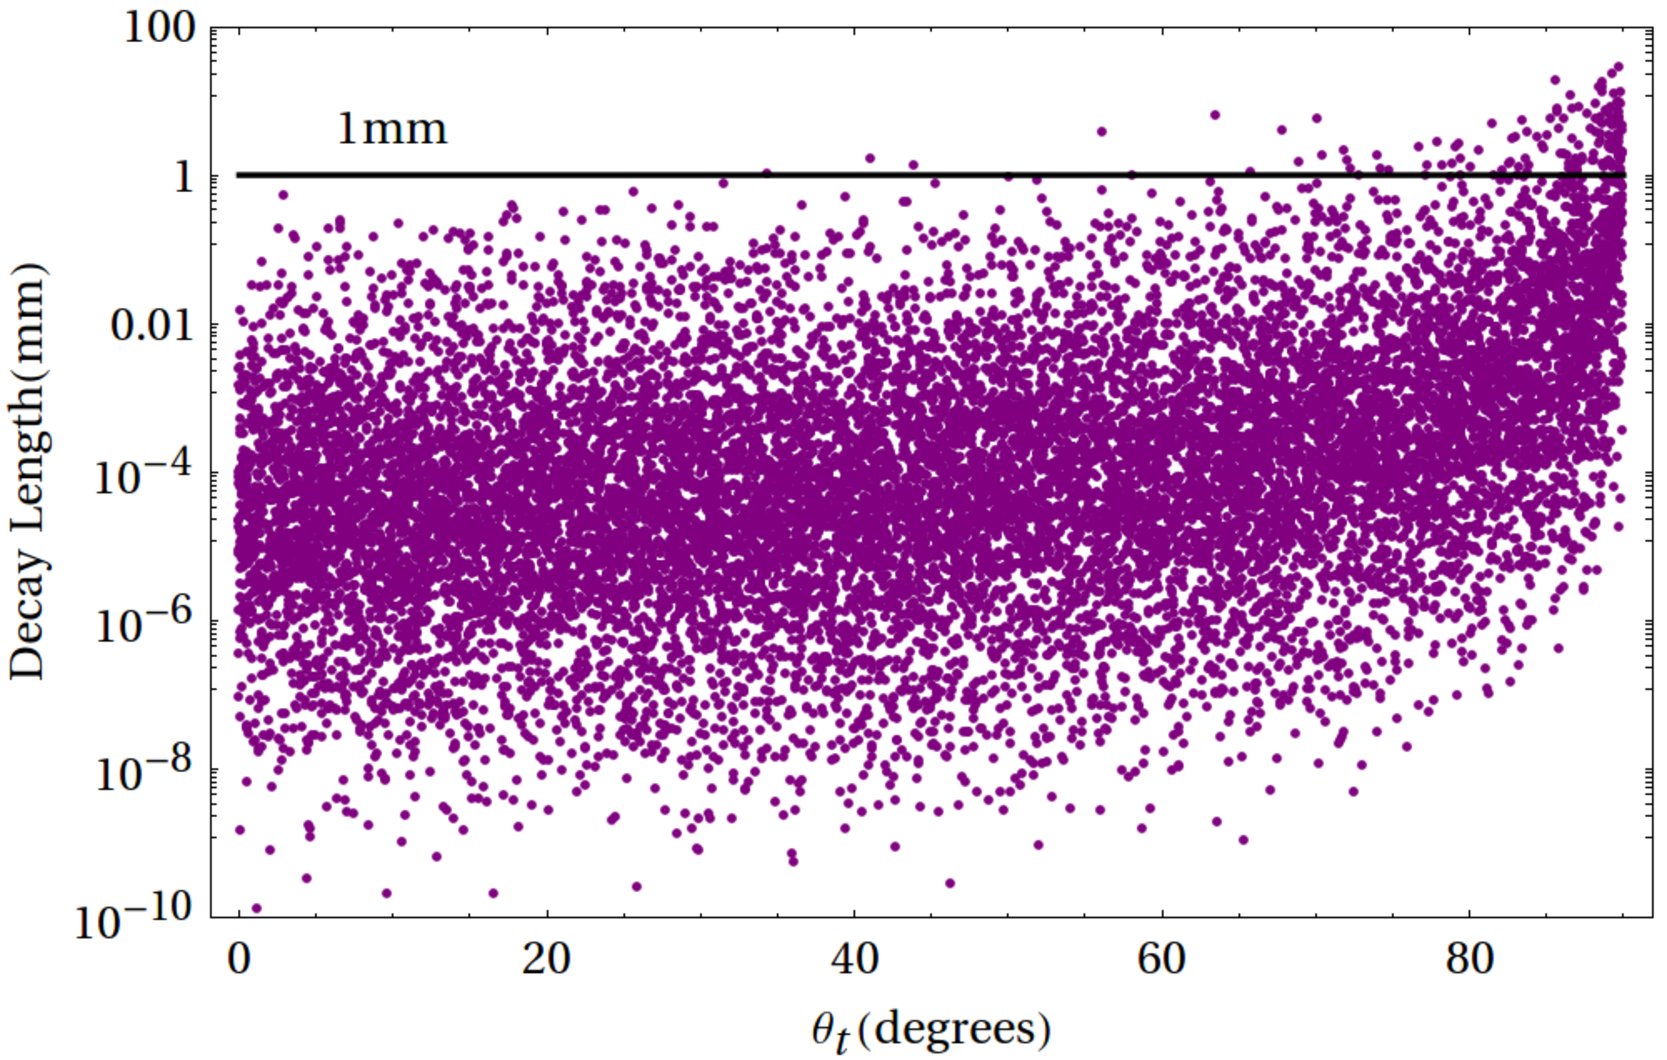
\includegraphics[width=\textwidth]{figs/theory/DecayLength.pdf}
      \label{fig:stop_decay_length_vs_mixing_angle}
    }
    \caption{These plots show the stop decay length and branching ratio versus
      the stop mixing angle, assuming the stop is the LSP.
      Each point in these plots represent a simulation with a particular
      choice of model parameters, which are varies within a range of natural
      values~\cite{Marshall:2014cwa}.
    }
    \label{fig:stop_vs_mixing_angle}
  }
\end{figure}

The analysis described in this thesis focuses on the $\stop \to b\ell$ decay
as it is preferred for most of parameter space.
Additionally, if the $\stop \to t\nu$ decay is significant, the decay of stop
pairs would lead to final states with $t\bar{t}$ associated with large missing
energy, which is the same final state as stop pair production with
$R$-Parity conserving decays, and the limits from traditional stop searches can
be reinterpreted for this model.

It is also reasonable to assume the stop decays in this model are prompt, and
decay with a negligible impact parameter, as shown in
Figure~\ref{fig:stop_decay_length_vs_mixing_angle}, where for most natural
models, the stop is expected to have a decay length of less than
$10^{-3}~\mathrm{mm}$;
in particular, this is true for models where the stop is not mostly
right-handed ($\theta_t \leq 80$)~\cite{Marshall:2014cwa,Marshall:2014kea}.
Therefore, long-lived particles are not considered in this analysis.

In this $B-L$ extension to the MSSM, stop pair production has the same
production cross section as in the traditional MSSM.
The expected production cross section are shown in Figure~\ref{fig:stop_xsec}.

\begin{figure}[ht]
  \centering{
    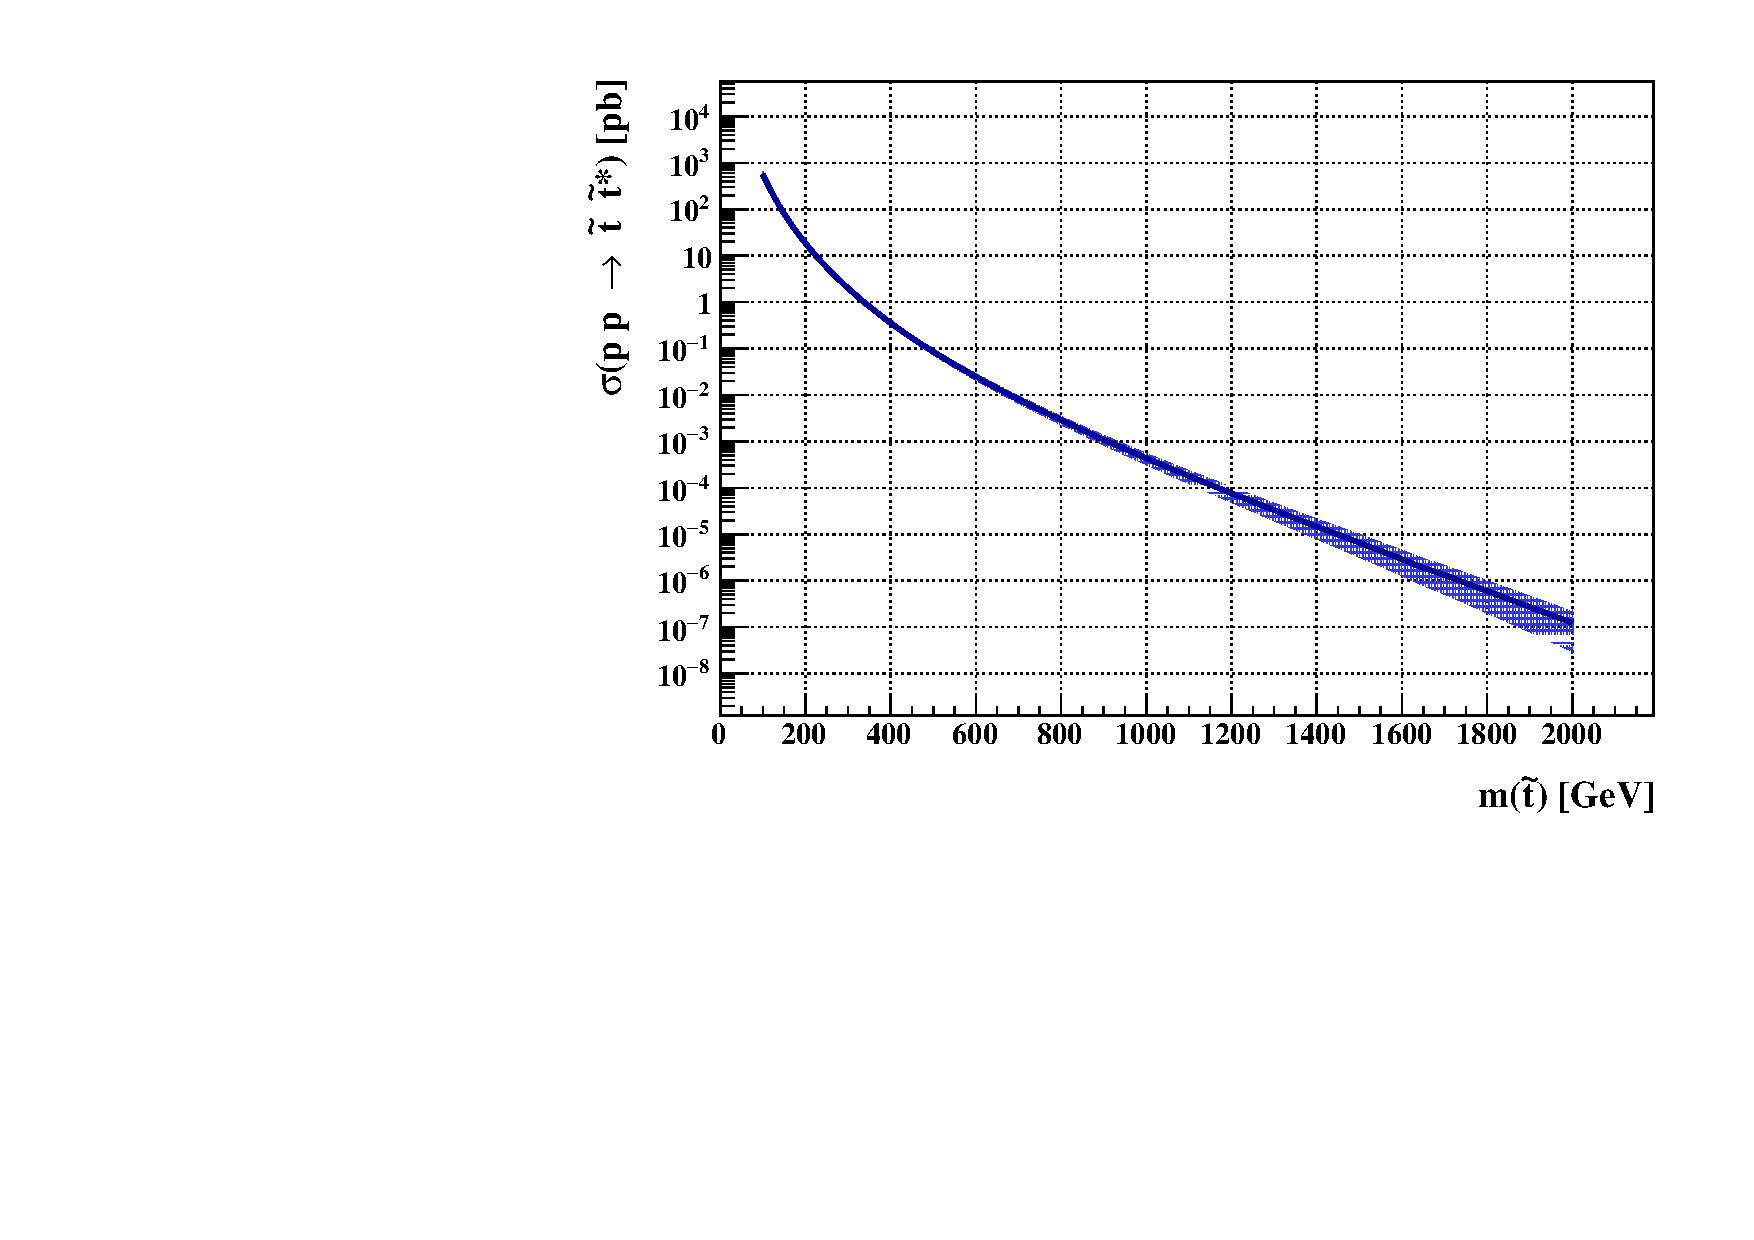
\includegraphics[width=\textwidth]{figs/theory/xsec.pdf}
  }
  \caption{Stop cross sections and their associated
    uncertainties~\cite{Beenakker:1997ut,Beenakker:2010nq,Beenakker:2011fu}.
  }
  \label{fig:stop_xsec}
\end{figure}

%% -----------------------------------------------------------------------------
\FloatBarrier
\subsection{Previous results}

The results from existing leptoquark searches performed at ATLAS were
re-interpreted in the context of this $B-L$ SUSY model with a stop LSP, and the
limits obtained on the minimum allowable stop mass across the plane of
physical stop branching ratios are shown in
Figure~\ref{fig:pheno_limit}~\cite{Marshall:2014cwa,Marshall:2014kea}.
The leptoquark searches, used to obtain these mass limits, searched for
models where the decay products are in the same generation.
As a result, $b$-tagging is only required in events associated with a $\tau$
lepton, and events with a light lepton simply require a jet, regardless of the
flavor.
Additionally, previous leptoquark searches only consider decays to a single
lepton flavor, resulting in final states with either two leptons of the same
flavor and two jets, or a single charged lepton and at least one jet.
The previous analyses did not consider final states with two charged leptons
with different flavors ($e\mu$) and at least two 
jets~\cite{ATLAS:2013oea, ATLAS:2012aq, Aad:2011ch, CMS:2014qpa,
  Chatrchyan:2012sv, Chatrchyan:2012vza, Chatrchyan:2012st}.
A dedicated search requiring $b$-tagged jets associated with light leptons
(electrons and muons), and considering different flavored leptons in the final
state can provide additional sensitivity to this model, as well as other models
which result in final states with $b$-quarks and light leptons in the final
state.

\begin{figure}[p]
  \centering{
    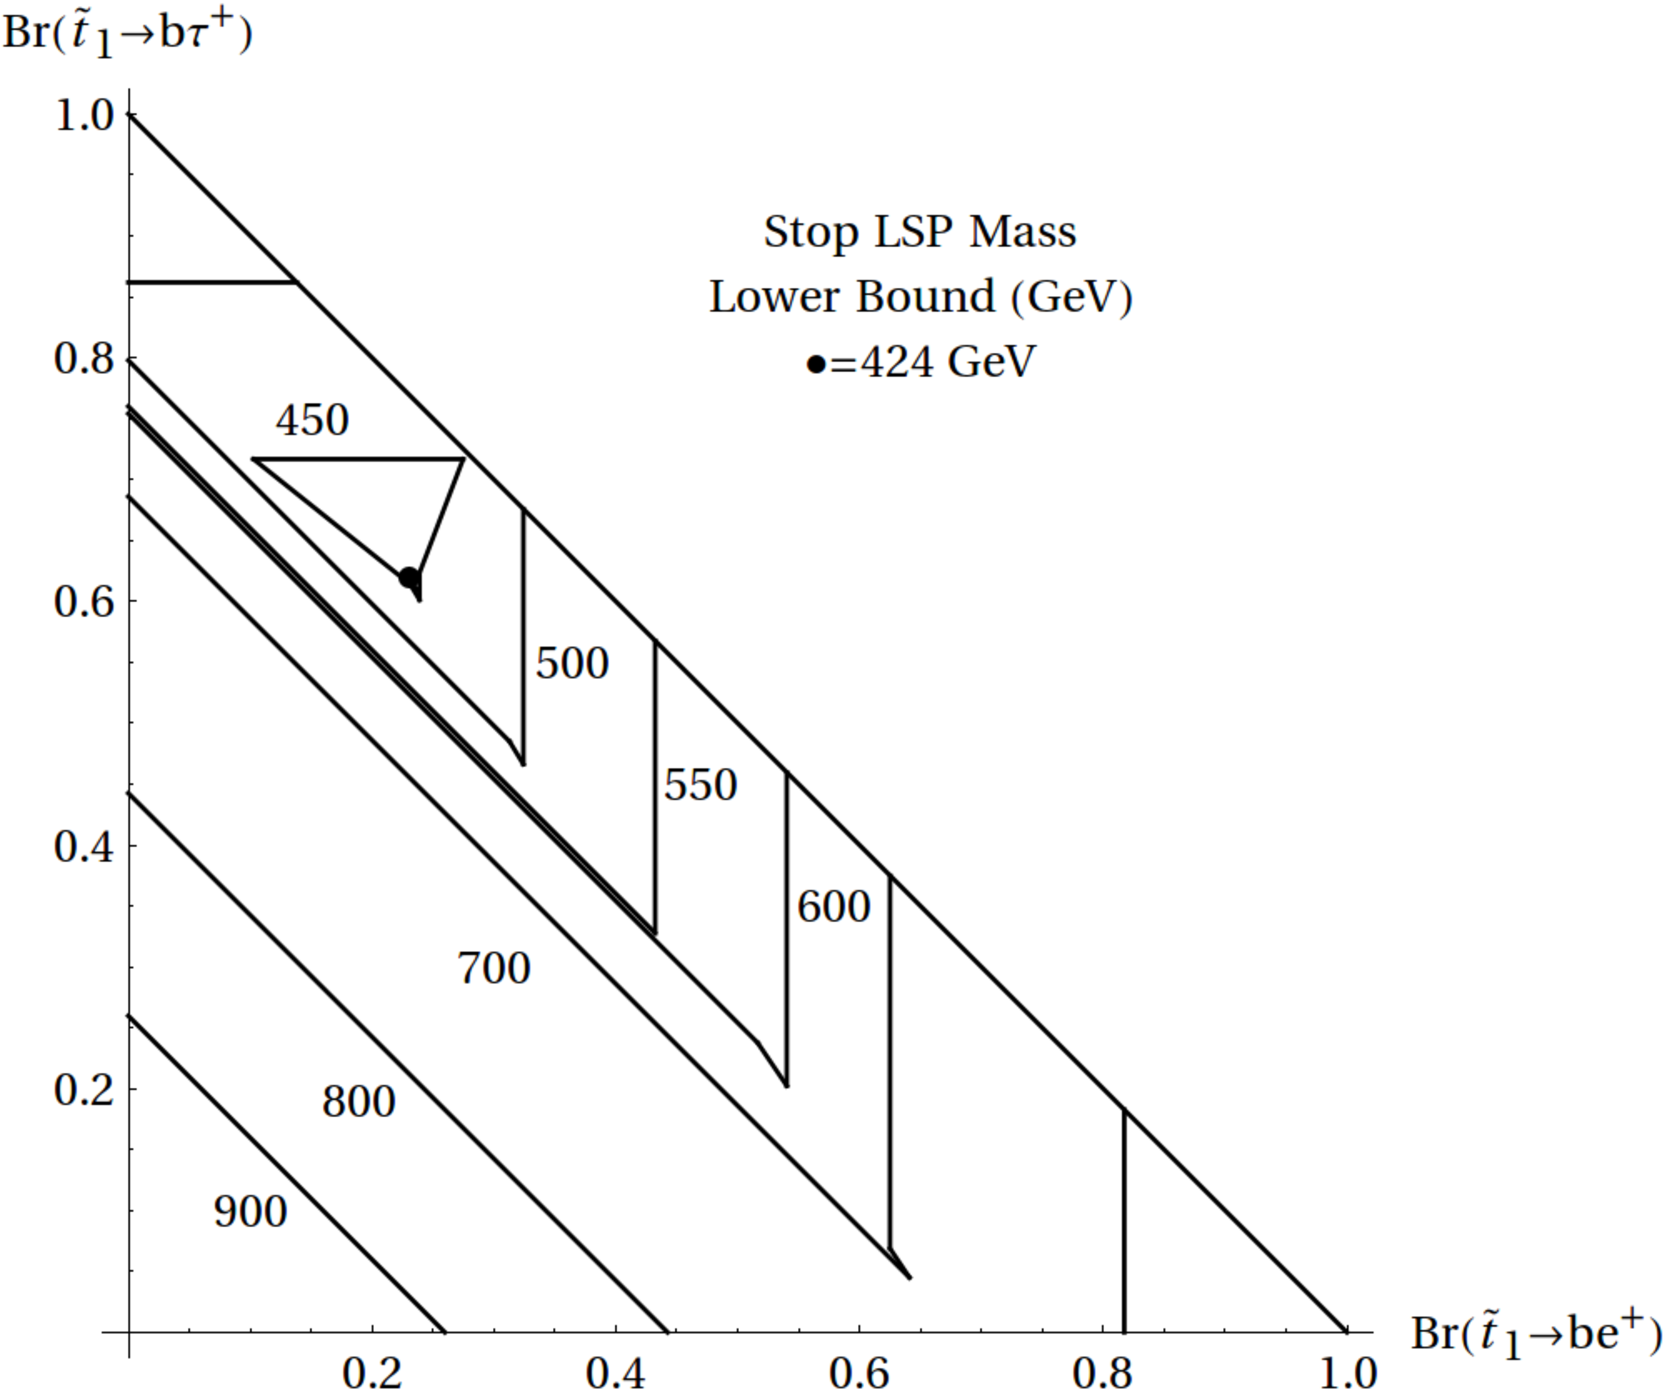
\includegraphics[width=\textwidth]
    {figs/theory/BoundContourPlotNoCombination.pdf}
    \caption{Limits on the stop mass obtained by reinterpreting leptoquark
      searches performed at ATLAS.
      The mass limits assume the stop is the LSP, and decays to a $b$-quark
      and a lepton~\cite{Marshall:2014cwa}.
    }
    \label{fig:pheno_limit}
  }
\end{figure}

